\documentclass[aspectratio=169,11pt,t]{beamer}
% ============================================================
%  ksa-cs-v2: ksa-cs-lecture-template.tex 스타일 + 한글, v2 덱(16:9)용.
%    - 짙은 네이비 헤드라인 (섹션 이름 + 프레임마다 점)
%    - 꽉 찬 파란 제목 막대, 둥근 그림자 블록
%    - 한글: Noto Sans CJK KR (fontspec)
%  사용:
%    \documentclass[aspectratio=169,11pt,t]{beamer}
%    \input{<..>/theme/ksa-cs-v2.tex}
%  ksa-theme.tex 의 매크로(\kb \kq, ksablue/ksared 등)도 같은 이름으로 둔다
%  -> v2 덱 본문을 거의 그대로 옮길 수 있다.
% ============================================================

\usepackage{fontspec}
\usepackage{amsmath,amssymb}
\usepackage{tikz}
\usepackage{listings}
\usepackage{graphicx}
\usepackage{booktabs}
\usepackage{varwidth}
% enumitem 은 넣지 않는다 (beamer 글머리표가 사라진다)

\defaultfontfeatures{Ligatures=TeX}
\setmainfont{Noto Sans CJK KR}
\setsansfont{Noto Sans CJK KR}
\setmonofont{Noto Sans Mono CJK KR}[Scale=0.92]
\usefonttheme{professionalfonts}

% ---------- 기본 틀 ----------
\usetheme{default}
\useinnertheme[shadow=true]{rounded}
\setbeamertemplate{navigation symbols}{}
\setbeamersize{text margin left=1em,text margin right=1em}

% ---------- 색 (템플릿 원본 값) ----------
\definecolor{navydark}{HTML}{191959}
\definecolor{navydim}{HTML}{8888B0}
\definecolor{navytitle}{HTML}{262686}
\definecolor{navyblue}{HTML}{3333B2}
\definecolor{blockbodybg}{HTML}{E9E9F3}
\definecolor{examplegreen}{HTML}{006000}
\definecolor{examplebg}{HTML}{E5EFE5}
\definecolor{alertred}{HTML}{BF0000}
\definecolor{alertbg}{HTML}{F9E5E5}
% ksa-theme.tex 와 같은 이름 (본문 호환)
\colorlet{ksablue}{navytitle}
\colorlet{ksabluedk}{navydark}
\definecolor{ksagold}{HTML}{D6CBB1}
\definecolor{ksagolddk}{HTML}{A9976B}
\colorlet{ksared}{alertred}
\definecolor{ksagray}{HTML}{5B5B5B}

\setbeamercolor{structure}{fg=navyblue}
\setbeamercolor{alerted text}{fg=alertred}
\setbeamercolor{frametitle}{bg=navytitle,fg=white}
\setbeamercolor{title}{fg=white,bg=navytitle}
\setbeamercolor{block title}{bg=navytitle,fg=white}
\setbeamercolor{block body}{bg=blockbodybg,fg=black}
\setbeamercolor{block title example}{bg=examplegreen,fg=white}
\setbeamercolor{block body example}{bg=examplebg,fg=black}
\setbeamercolor{block title alerted}{bg=alertred,fg=white}
\setbeamercolor{block body alerted}{bg=alertbg,fg=black}
\setbeamercolor{item}{fg=navyblue}
\setbeamertemplate{itemize item}[circle]
\setbeamertemplate{itemize subitem}[triangle]

% ---------- 헤드라인: miniframes (섹션 이름 + 점) ----------
\useoutertheme[subsection=false]{miniframes}
\setbeamerfont{section in head/foot}{size=\tiny}
\setbeamercolor{section in head/foot}{bg=navydark,fg=white}
\setbeamercolor{mini frame}{fg=white}
\setbeamertemplate{mini frames}[circle]

% ---------- 제목 막대: 폭 꽉 채움, 두 줄까지 ----------
\setbeamerfont{frametitle}{size=\normalsize,series=\bfseries}
\setbeamertemplate{frametitle}{%
  \nointerlineskip
  \begin{beamercolorbox}[wd=\paperwidth,ht=2.7ex,dp=1.1ex,leftskip=.3cm,rightskip=.3cm]{frametitle}%
    \usebeamerfont{frametitle}\insertframetitle
  \end{beamercolorbox}}

% ---------- 쪽 번호: 오른쪽 아래 ----------
\setbeamertemplate{footline}{%
  \hfill
  {\color{navydim}\scriptsize\insertframenumber\,/\,\inserttotalframenumber}%
  \hspace{3mm}\vspace{2mm}%
}

% ---------- 표지: 템플릿처럼 헤드라인은 그대로, 가운데 둥근 그림자 상자에 제목 한 줄 ----------
% 덱에서:  {\setbeamertemplate{footline}{}\begin{frame}[c,noframenumbering]\titlepage\end{frame}}
\setbeamercolor{title}{fg=white,bg=navyblue}
\makeatletter
\setbeamertemplate{title page}{%
  \vfill
  \centering
  \begin{minipage}{0.84\paperwidth}
  \begin{beamercolorbox}[wd=\linewidth,sep=7pt,center,rounded=true,shadow=true]{title}
    {\usebeamerfont{title}\inserttitle\par}%
    \ifx\insertsubtitle\@empty\else\vskip0.4em{\usebeamerfont{subtitle}\insertsubtitle\par}\fi
  \end{beamercolorbox}
  \end{minipage}\par\vskip1.6em
  {\usebeamerfont{author}\color{navytitle}\insertauthor\par}\ifx\beamer@date\@empty\vskip0.3em\else\vskip1.3em\fi
  {\usebeamerfont{institute}\color{ksagray}\insertinstitute\par}%
  \ifx\beamer@date\@empty\else\vskip0.3em{\usebeamerfont{date}\color{ksagray}\insertdate\par}\fi
  \vfill
}
\makeatother
\setbeamerfont{title}{series=\bfseries,size=\Large}
\setbeamerfont{subtitle}{size=\normalsize}
\setbeamerfont{author}{size=\normalsize}
\setbeamerfont{institute}{size=\small}
\setbeamerfont{date}{size=\small}

% ksa-theme 호환: 덱이 \renewcommand{\ksacredit}{..} 를 해도 되게 (꼬리말에는 안 쓴다)
\newcommand{\ksacredit}{}

% ---------- 강조 ----------
\newcommand{\hl}[1]{\textcolor{alertred}{#1}}
\newcommand{\hlb}[1]{\textcolor{navyblue}{#1}}
\newcommand{\kb}[1]{\textbf{\color{ksablue}#1}}
\newcommand{\kq}[1]{\textbf{\color{ksared}#1}}

% ---------- 파이썬 코드 (템플릿과 같은 색) ----------
\definecolor{codekw}{HTML}{0033B3}
\definecolor{codebuiltin}{HTML}{BF0000}
\definecolor{codestr}{HTML}{067D17}
\definecolor{codecomment}{HTML}{8C8C8C}
\definecolor{codenum}{HTML}{1750EB}
\lstdefinestyle{py}{
  language=Python, basicstyle=\ttfamily\scriptsize,
  keywordstyle=\color{codekw}\bfseries, stringstyle=\color{codestr},
  commentstyle=\color{codecomment}\itshape, numberstyle=\color{codenum},
  emph={print,len,range,sum,input,int,str,float,list,dict,append,remove,sorted,abs,min,max},
  emphstyle=\color{codebuiltin}, showstringspaces=false, keepspaces=true,
  columns=fixed, basewidth=0.52em, aboveskip=1mm, belowskip=1mm, xleftmargin=2mm,
  breaklines=true
}
\lstset{style=py}

% 원본 덱 (ksa-theme) 의 그림·실습은 이 폴더로 합쳤다 (옛 원본: slides/old/v2/)
\setbeamerfont{author}{size=\normalsize}
\setbeamerfont{institute}{size=\small}
\graphicspath{{figs/}{../../../assets/}}
\makeatletter
\newcommand{\markpage}[1]{\protected@write\@auxout{}{\string\newlabel{#1}{{\the\c@framenumber}{}}}\hypertarget{#1}{}}
\newcommand{\pref}[1]{\hyperlink{#1}{\textcolor{ksagolddk}{(p.\ref{#1})}}}
\makeatother

\renewcommand{\ksacredit}{Machine Learning and Deep Learning \,\textperiodcentered\, 서포트 벡터 머신}
\title{서포트 벡터 머신 (Support Vector Machine)}
\subtitle{가장 넓은 길을 내는 분류기, 그리고 커널 트릭}
\author{Machine Learning and Deep Learning}
\institute{KSA 2027-Spring}
\date{Sumin Han (suminhan@ksa.hs.kr)}
\begin{document}
{\setbeamertemplate{footline}{}\begin{frame}[c,noframenumbering]\titlepage\end{frame}}

\section{질문}
% --- 오늘의 질문
\begin{frame}{오늘의 질문}
\vfill
\begin{columns}[c]
\begin{column}{0.44\textwidth}\centering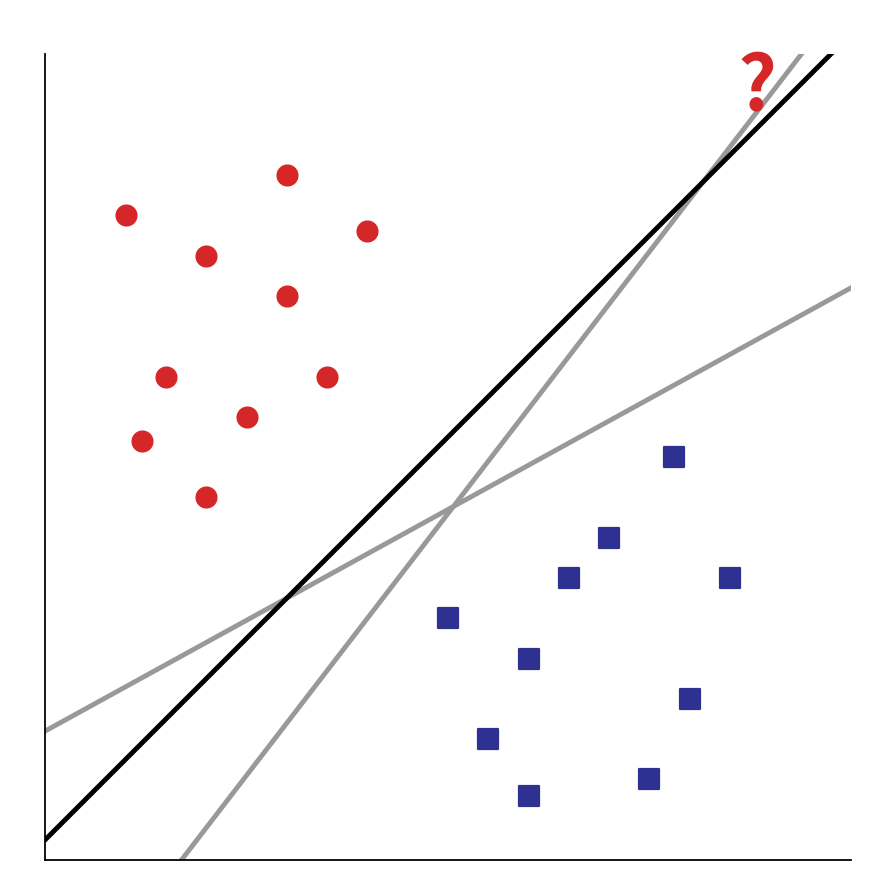
\includegraphics[width=0.95\linewidth]{sv_hook.png}\end{column}
\begin{column}{0.52\textwidth}
{\Large 빨강과 파랑을 가르는 직선}\\[0.8em]
{\large 세 선 모두 학습 데이터를 \textbf{완벽하게} 가른다}\\[0.8em]
{\Large \kq{어느 선이 가장 좋을까?}}
\end{column}
\end{columns}
\vfill
\note{빨간 점과 파란 점이 있습니다. 둘을 가르는 직선을 세 개 그었는데, 세 선 모두 학습 데이터를 하나도 틀리지 않고 완벽하게 가릅니다. 학습 오차로는 셋 다 0입니다. 그런데 어느 선이 가장 좋을까요? 직관적으로는 가운데 검은 선이 가장 안심이 됩니다. 왜 그런지, 그리고 그 선을 어떻게 찾는지가 오늘의 주제입니다.}
\end{frame}

\section{마진}
% --- 바짝 붙은 선
\begin{frame}{점에 바짝 붙은 선은 위험하다}
\vfill
\begin{columns}[c]
\begin{column}{0.44\textwidth}\centering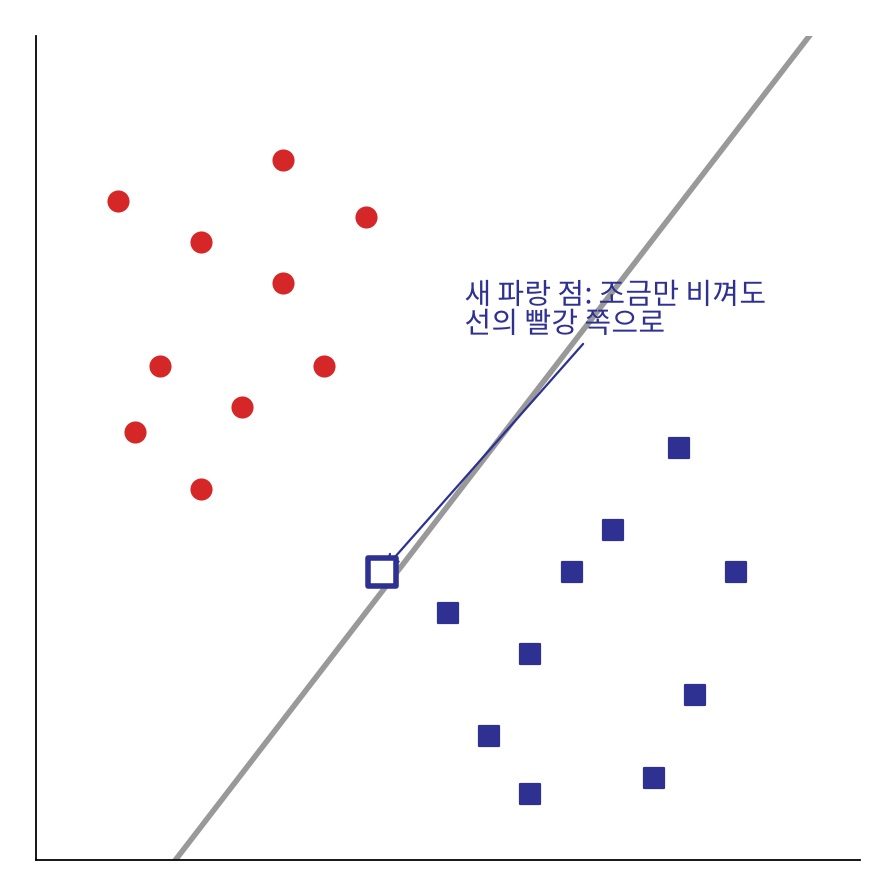
\includegraphics[width=0.95\linewidth]{sv_risky.png}\end{column}
\begin{column}{0.52\textwidth}
{\large 가르는 선은 \textbf{무수히} 많다}\\[0.8em]
{\large 점에 바짝 붙은 선은 새 점이\\ 조금만 비껴 와도 \kq{틀린다}}\\[0.8em]
{\large 양쪽에서 \kb{가장 멀리} 떨어진 선이 안전하다}
\end{column}
\end{columns}
\vfill
\note{가르는 직선은 사실 무수히 많습니다. 그중 파란 점에 바짝 붙은 선을 보세요. 학습 데이터는 맞히지만, 파란 무리 근처에서 새 파란 점이 조금만 위로 비껴 오면 선의 빨강 쪽으로 넘어가서 틀립니다. 측정 오차나 개인차로 새 데이터는 늘 조금씩 비껴 옵니다. 그래서 양쪽 무리에서 가장 멀리 떨어진 선, 양쪽에 여유를 가장 많이 남기는 선이 안전합니다.}
\end{frame}

% --- 가장 넓은 길
\begin{frame}{SVM: 가장 넓은 길을 낸다}
\markpage{street}
\vfill
\begin{columns}[c]
\begin{column}{0.44\textwidth}\centering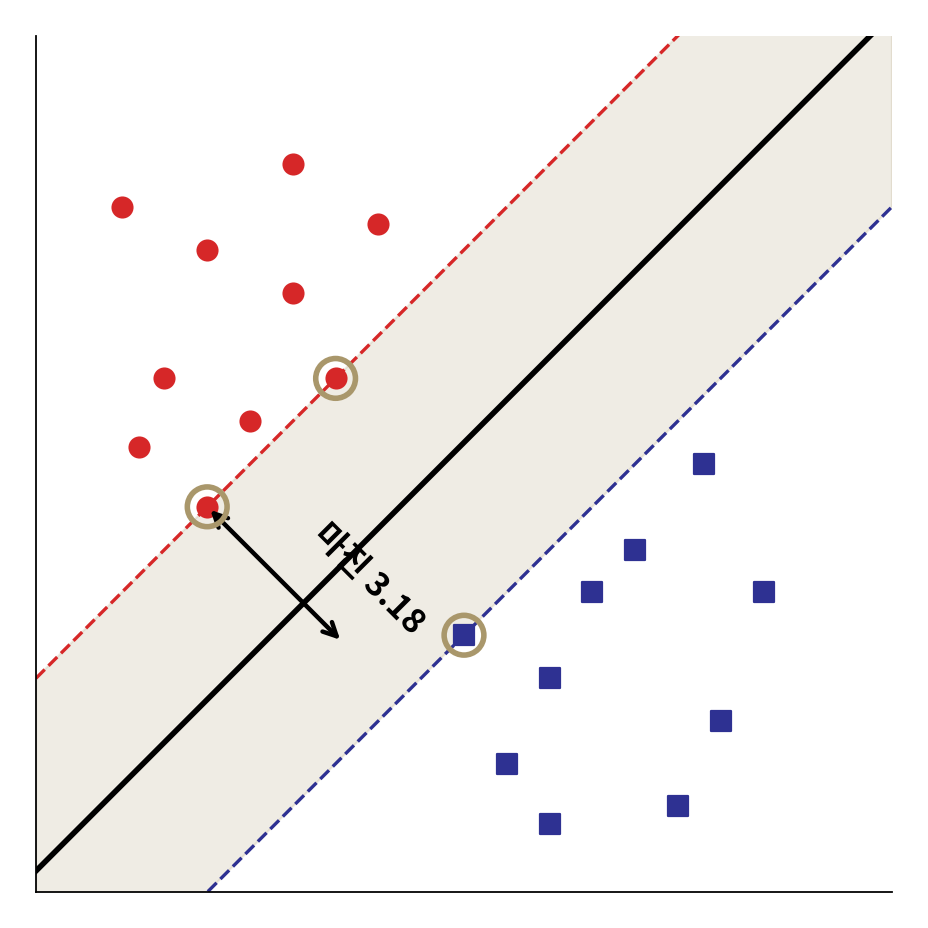
\includegraphics[width=0.95\linewidth]{sv_street.png}\end{column}
\begin{column}{0.52\textwidth}
{\large 두 무리 사이에 \textbf{길}을 낸다}\\[0.6em]
{\large 길의 폭 = \kb{마진 (margin)}}\\[0.6em]
{\large SVM: 마진이 \textbf{가장 넓은} 길의 가운데 선}\\[0.8em]
{\large 이 데이터: 마진 \kb{3.18}}\\[0.4em]
{\small 길 가장자리 (점선) 에 닿은 점 = \textbf{서포트 벡터} (노란 동그라미)}
\end{column}
\end{columns}
\vfill
\note{서포트 벡터 머신, SVM은 두 무리 사이에 길을 냅니다. 길 안에는 점이 하나도 없어야 하고, 길의 폭을 마진이라고 부릅니다. SVM은 마진이 가장 넓은 길을 찾고, 그 길의 가운데 선을 경계로 씁니다. 이 데이터에서 가장 넓은 길의 폭은 3.18입니다. 길 가장자리, 점선에 딱 닿은 점들이 노란 동그라미로 표시돼 있습니다. 이 점들을 서포트 벡터라고 부르고, 이름이 여기서 나왔습니다.}
\end{frame}

% --- 식 읽기 2: 점곱
\begin{frame}{식 읽기 \textcircled{1}: $\mathbf{w}\cdot\mathbf{x}$ = 자리끼리 곱해서 더하기}
\vfill
\centering
{\LARGE $\mathbf{w}\cdot\mathbf{x} + b \;=\; w_1 x_1 + w_2 x_2 + b$}\\[0.3em]
{\large $\mathbf{x} = (x_1, x_2)$: 점 \kb{하나}의 좌표 \quad $\mathbf{w} = (w_1, w_2)$: 가중치 \quad $b$: 숫자 하나}\\[0.6em]
\renewcommand{\arraystretch}{1.35}
{\large\begin{tabular}{c|c|c}
점 $\mathbf{x}$ & $\mathbf{w} = (1, 1),\ b = -3$ & 점수\\ \hline
$(3, 2)$ & $1{\cdot}3 + 1{\cdot}2 - 3$ & \textcolor{ksared}{$\mathbf{+2}$}\\
$(1, 2)$ & $1{\cdot}1 + 1{\cdot}2 - 3$ & $\mathbf{0}$\\
$(1, 1)$ & $1{\cdot}1 + 1{\cdot}1 - 3$ & \textcolor{ksablue}{$\mathbf{-1}$}
\end{tabular}}\\[0.8em]
{\large 로지스틱회귀의 $z = w_0 + w_1 x_1 + w_2 x_2$ 와 \kb{같은 식} (절편 $w_0$ 을 $b$ 라고 부를 뿐)}
\vfill
\note{굵은 글자 x는 점 하나의 좌표 두 개, w는 가중치 두 개를 묶은 것이고, b는 숫자 하나입니다. x는 데이터 전체가 아니라 점 하나입니다. 세로 좌표를 y라고 하지 않는 이유는 y를 점의 색, 라벨에 쓰기 때문입니다. 점곱을 하면 숫자 하나가 나오니까 거기에 숫자 하나 b를 더할 수 있습니다. 가운데 점은 점곱이라고 읽고, 계산은 간단합니다. 같은 자리끼리 곱해서 모두 더합니다. w1 곱하기 x1 더하기 w2 곱하기 x2, 여기에 b를 더하면 점수 하나가 나옵니다. w가 1, 1이고 b가 마이너스 3일 때 점 3, 2를 넣으면 3 더하기 2 빼기 3, 플러스 2입니다. 점 1, 2는 0, 점 1, 1은 마이너스 1입니다. 사실 처음 보는 식이 아닙니다. 로지스틱회귀에서 체스 레이팅 두 개로 z를 계산한 식, w0 더하기 w1 x1 더하기 w2 x2와 똑같습니다. 특징마다 가중치를 곱해서 더하고 절편을 더한 점수입니다. 절편 w0을 SVM에서는 b라고 부를 뿐입니다.}
\end{frame}

% --- 식 읽기 3: 점수 지도
\begin{frame}{식 읽기 \textcircled{2}: 점수가 0 인 점을 이으면 직선}
\vfill
\begin{columns}[c]
\begin{column}{0.46\textwidth}\centering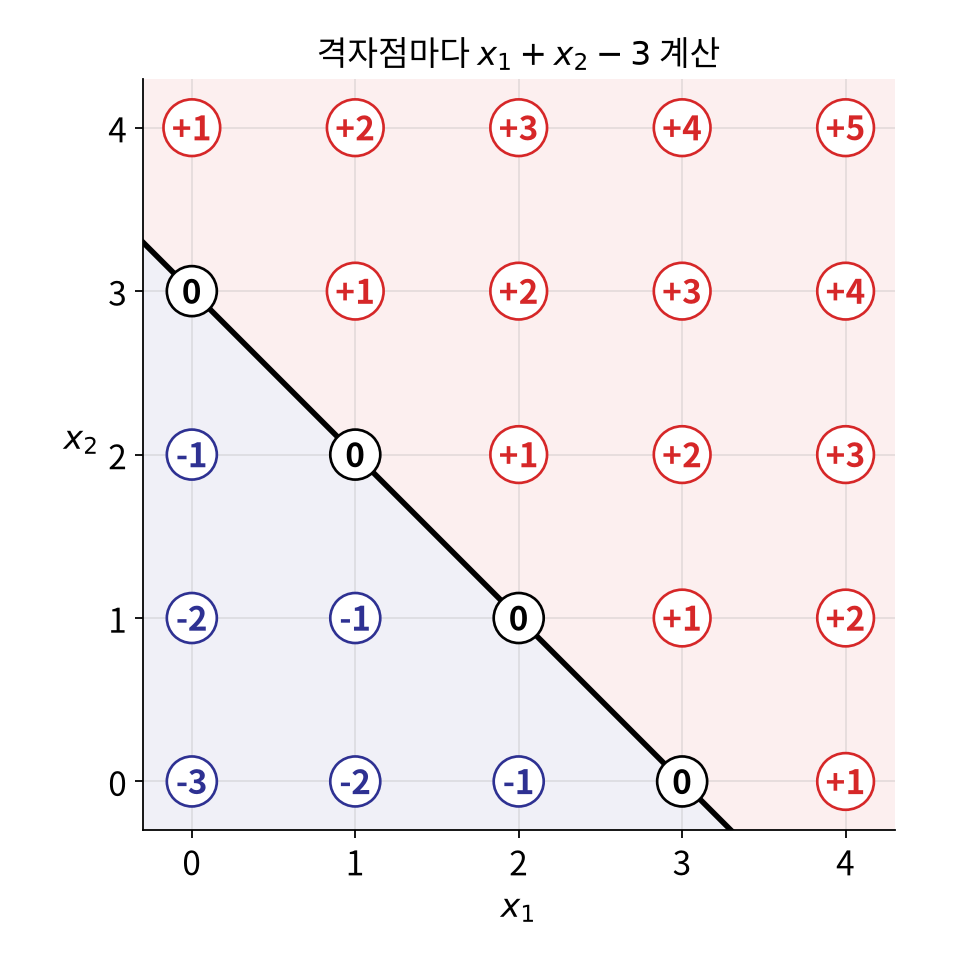
\includegraphics[width=0.88\linewidth]{sv_scoremap.png}\end{column}
\begin{column}{0.50\textwidth}
{\large 평면의 모든 점에 점수가 붙는다}\\[0.8em]
{\large 점수 \textcolor{ksared}{$+$} 쪽 \;/\; \textcolor{ksablue}{$-$} 쪽 \;/\; \textbf{0} 인 곳}\\[0.8em]
{\large $x_1 + x_2 - 3 = 0$}\\[0.2em]
{\large $\Leftrightarrow$ \kb{$x_2 = -x_1 + 3$} (중학교 직선)}\\[0.8em]
{\large 경계 $\mathbf{w}\cdot\mathbf{x} + b = 0$ = \kq{점수 0 인 선}}
\end{column}
\end{columns}
\vfill
\note{이제 평면의 격자점마다 이 점수를 계산해서 적어 봤습니다. 오른쪽 위로 갈수록 점수가 커지고, 왼쪽 아래로 갈수록 작아집니다. 점수가 정확히 0인 점들, 0, 3과 1, 2와 2, 1과 3, 0을 이으면 직선이 됩니다. x1 더하기 x2 빼기 3이 0이라는 식을 x2에 대해 풀면 x2 등호 마이너스 x1 더하기 3, 중학교 때 본 기울기 마이너스 1, y절편 3인 직선입니다. 그래서 SVM의 경계 w 점곱 x 더하기 b 등호 0은 점수가 0인 선이라는 뜻입니다. 점수가 양수인 쪽은 빨강, 음수인 쪽은 파랑으로 분류합니다.}
\end{frame}

% --- 식 읽기 4: w 는 수직
\begin{frame}{식 읽기 \textcircled{3}: $\mathbf{w}$ 는 경계에 수직인 오르막}
\vfill
\begin{columns}[c]
\begin{column}{0.46\textwidth}\centering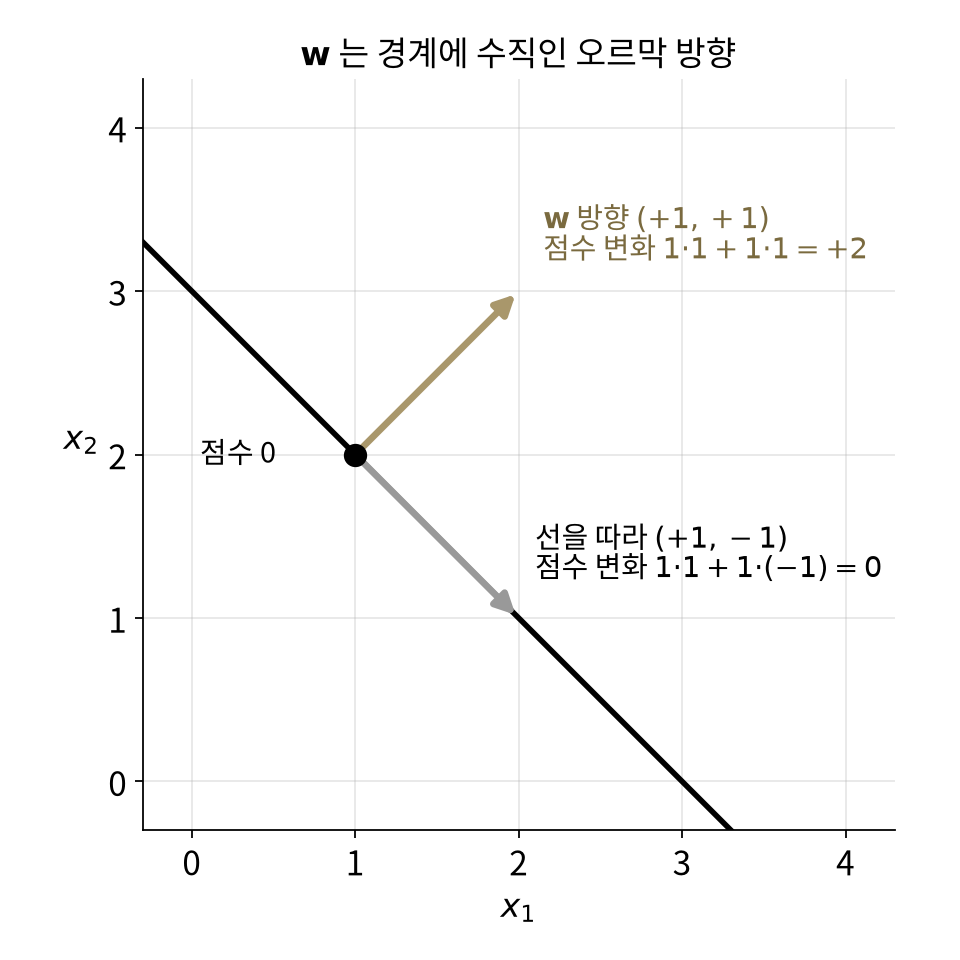
\includegraphics[width=0.88\linewidth]{sv_perp.png}\end{column}
\begin{column}{0.50\textwidth}
{\large 경계 위 점 $(1, 2)$ 에서 출발}\\[0.8em]
{\large 선을 따라 $(+1, -1)$: 점수 변화 \textbf{0}}\\[0.3em]
{\large $\mathbf{w}$ 방향 $(+1, +1)$: 점수 변화 \textcolor{ksared}{$\mathbf{+2}$}}\\[0.8em]
{\large $\mathbf{w}$ = 점수가 \kb{가장 빨리 오르는 방향}}\\[0.2em]
{\large = 경계에 \kb{수직}}
\end{column}
\end{columns}
\vfill
\note{w라는 화살표가 그림에서 어디를 가리키는지 봅시다. 경계 위의 점 1, 2에서 출발합니다. 경계를 따라 오른쪽으로 1, 아래로 1 움직이면 점수 변화는 1 곱하기 1 더하기 1 곱하기 마이너스 1, 0입니다. 선 위에서는 아무리 움직여도 점수가 그대로입니다. 반면 w 방향, 오른쪽으로 1, 위로 1 움직이면 점수가 2 오릅니다. 같은 거리를 걸을 때 점수가 가장 빨리 오르는 방향이 w이고, 그 방향은 경계와 직각입니다. 등고선과 오르막 방향의 관계와 같습니다. 다음 쪽부터 나오는 w는 모두 경계에 수직인 이 화살표입니다.}
\end{frame}

% --- ±1 은 약속
\begin{frame}{가장자리는 왜 $\pm 1$ 일까: 크기를 맞추는 약속}
\markpage{scale}
\vfill
\centering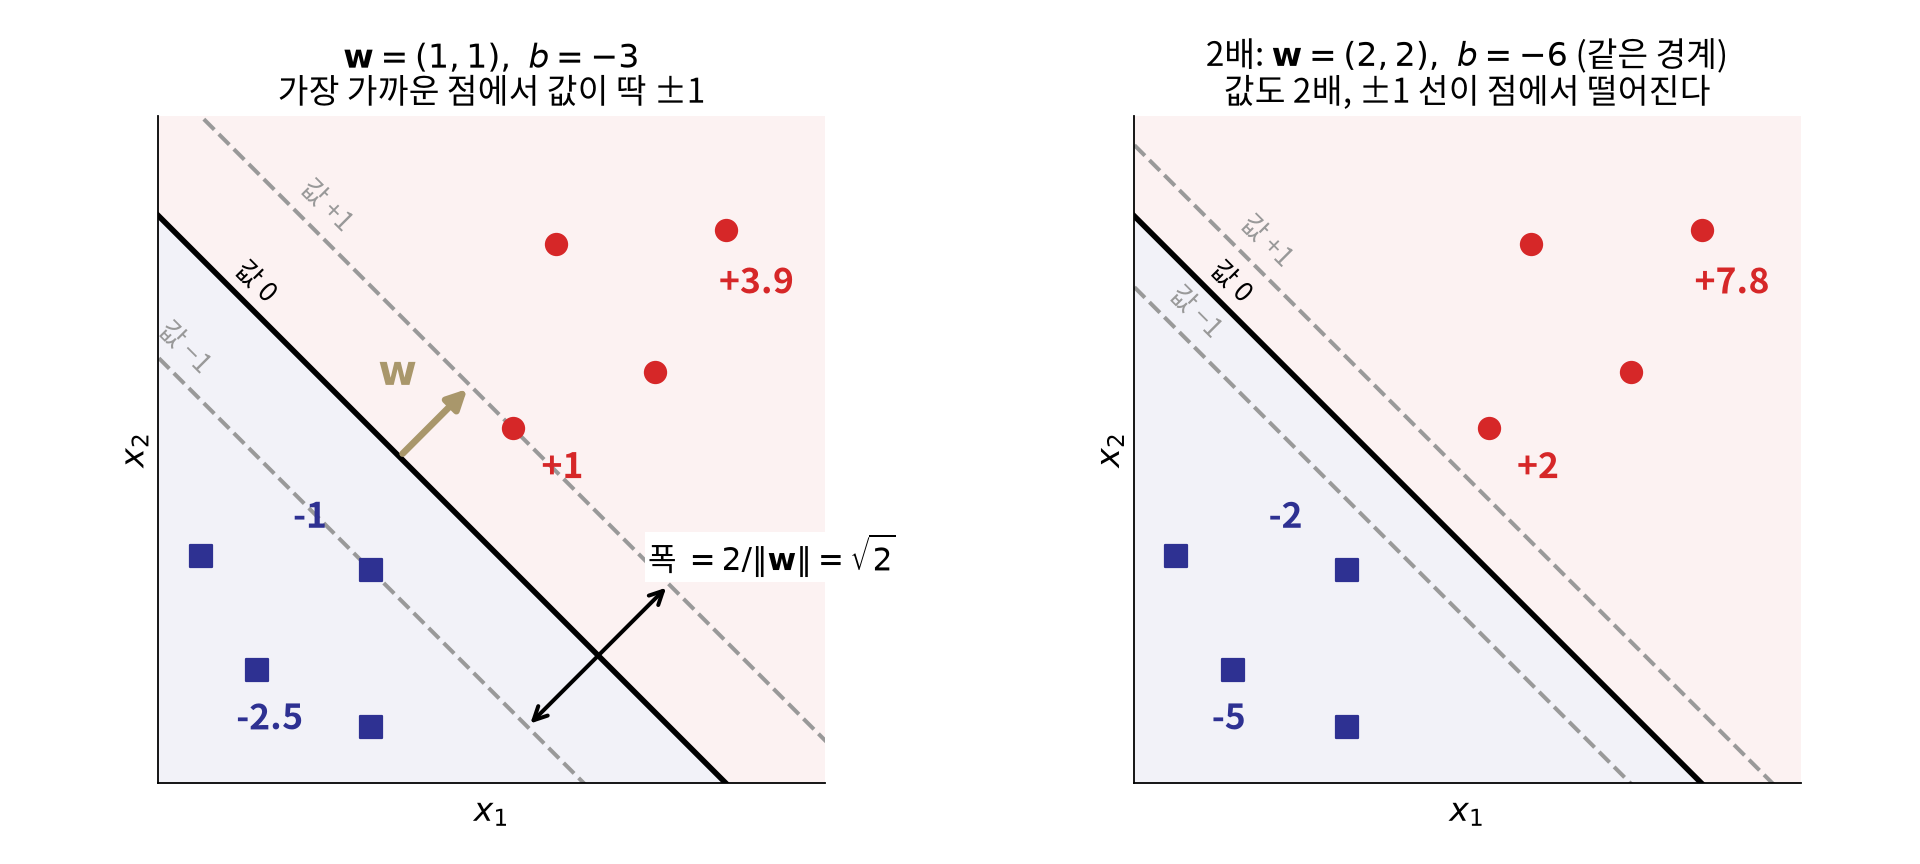
\includegraphics[width=0.7\linewidth]{sv_scale.png}\par\vskip0.2em
{\normalsize \textbf{1.} 경계 $\mathbf{w}\cdot\mathbf{x} + b = 0$: 값이 \textcolor{ksared}{$+$ 면 빨강}, \textcolor{ksablue}{$-$ 면 파랑}. $\mathbf{w}$ 는 경계에 수직}\\[0.2em]
{\normalsize \textbf{2.} $(\mathbf{w}, b)$ 를 2배 해도 \textbf{같은 경계} $\to$ 가장 가까운 점에서 값이 $\pm 1$ 이 되게 \kb{크기를 정한다}}\\[0.2em]
{\normalsize \textbf{3.} 점에서 경계까지 거리 $= |\mathbf{w}\cdot\mathbf{x} + b| \,/\, \lVert\mathbf{w}\rVert$ $\to$ 가장자리는 $1/\lVert\mathbf{w}\rVert$, 폭은 \kb{$2/\lVert\mathbf{w}\rVert$}}
\vfill
\note{길을 식으로 쓰기 전에, 가장자리가 왜 플러스 마이너스 1인지 봅시다. 왼쪽 그림의 검은 선은 x1 더하기 x2 빼기 3이 0인 직선, w는 1, 1이고 b는 마이너스 3입니다. 점을 넣어 이 값을 계산하면 빨간 점은 양수, 파란 점은 음수입니다. 그래서 값의 부호로 분류합니다. w는 이 경계에 수직인 방향입니다. 그런데 오른쪽처럼 w와 b를 둘 다 2배 해도, 2 x1 더하기 2 x2 빼기 6이 0인 직선은 똑같은 선입니다. 값만 2배가 될 뿐입니다. 경계는 같은데 식을 쓰는 방법이 무수히 많은 겁니다. 그래서 하나로 정하는 약속을 합니다. 경계에 가장 가까운 점에서 값이 딱 플러스 1, 마이너스 1이 되도록 크기를 맞춘다. 왼쪽이 그렇게 맞춘 것이고, 그래서 가장자리 점선이 값 플러스 1, 마이너스 1인 선입니다. 오른쪽처럼 2배 하면 값 플러스 마이너스 1인 선이 점에서 떨어져 버립니다. 마지막으로 점에서 직선까지의 거리는 값의 절댓값을 w의 길이로 나눈 것입니다. 가장자리 위의 점은 값이 1이니 경계까지 1 나누기 w의 길이, 양쪽을 합친 길의 폭은 2 나누기 w의 길이입니다. 이 예에서는 w의 길이가 루트 2라서 폭이 루트 2, 두 점 1, 1과 2, 2 사이의 거리와 같습니다.}
\end{frame}

% --- 왜 폭이 2/||w|| 인가 (1): 걸어 보기
\begin{frame}{가장자리까지 몇 걸음? $\mathbf{w}$ 방향으로 걸어 보면}
\vfill
\begin{columns}[c]
\begin{column}{0.40\textwidth}\centering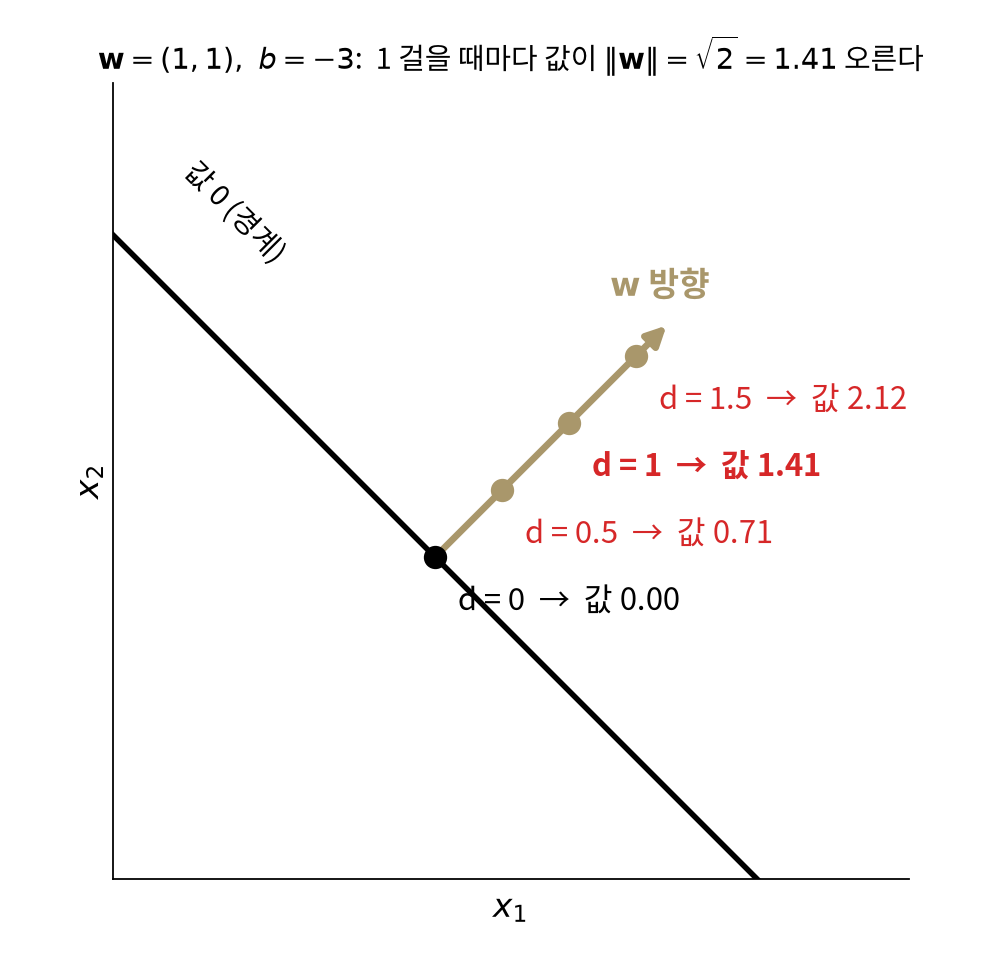
\includegraphics[width=\linewidth]{sv_walk.png}\end{column}
\begin{column}{0.58\textwidth}
{\large \textbf{1.} 경계 위 점 $\mathbf{x}_0$ 에서 값 $= 0$}\\[0.6em]
{\large \textbf{2.} $\mathbf{w}$ 방향 (길이 1: $\mathbf{u} = \mathbf{w}/\lVert\mathbf{w}\rVert$) 으로 $d$ 걸으면}\\[0.3em]
{\normalsize $\mathbf{w}\cdot(\mathbf{x}_0 + d\,\mathbf{u}) + b \;=\; \underbrace{\mathbf{w}\cdot\mathbf{x}_0 + b}_{0} \;+\; d\,\underbrace{\mathbf{w}\cdot\mathbf{u}}_{\lVert\mathbf{w}\rVert} \;=\;$ \kb{$d\,\lVert\mathbf{w}\rVert$}}\\[0.6em]
{\large \textbf{3.} 값이 $+1$ 이 되는 곳: \kb{$d = 1/\lVert\mathbf{w}\rVert$}}\\[0.3em]
{\normalsize $\lVert\mathbf{w}\rVert$ = 화살표 $\mathbf{w}$ 의 길이 $= \sqrt{w_1^2 + w_2^2}$}\\[0.2em]
{\normalsize 예: $\sqrt{1^2 + 1^2} = 1.41$ $\to$ $d = 0.71$}
\end{column}
\end{columns}
\vfill
\note{가장자리 값을 플러스 마이너스 1로 정했는데, 그게 왜 폭 2 나누기 w의 길이가 되는지 걸어 보면서 확인합니다. 앞 쪽의 예, w가 1, 1이고 b가 마이너스 3인 경계입니다. 경계 위 점 1.5, 1.5에서 값은 0입니다. 여기서 w 방향, 즉 경계에 수직인 방향으로 걸어 봅니다. 0.5 걸으면 값이 0.71, 1 걸으면 1.41, 1.5 걸으면 2.12. 1 걸을 때마다 값이 1.41씩, 정확히 w의 길이 루트 2만큼 오릅니다. 식으로 보면, w를 자기 길이로 나눈 길이 1짜리 방향 u를 d배 해서 x0에 더하고 값을 계산하면, 앞부분은 경계 위라서 0이고, 뒷부분 w 점곱 u는 w 길이의 제곱을 w 길이로 나눈 것, 즉 w의 길이입니다. 그래서 d 곱하기 w의 길이가 남습니다. 그러면 값이 1이 되는 곳, 가장자리는 d가 1 나누기 w의 길이인 곳입니다. 이 예에서는 0.71 걸으면 가장자리입니다.}
\end{frame}

% --- 왜 폭이 2/||w|| 인가 (2)
\begin{frame}{그래서 폭 $= 2/\lVert\mathbf{w}\rVert$}
\markpage{width}
\vfill
\centering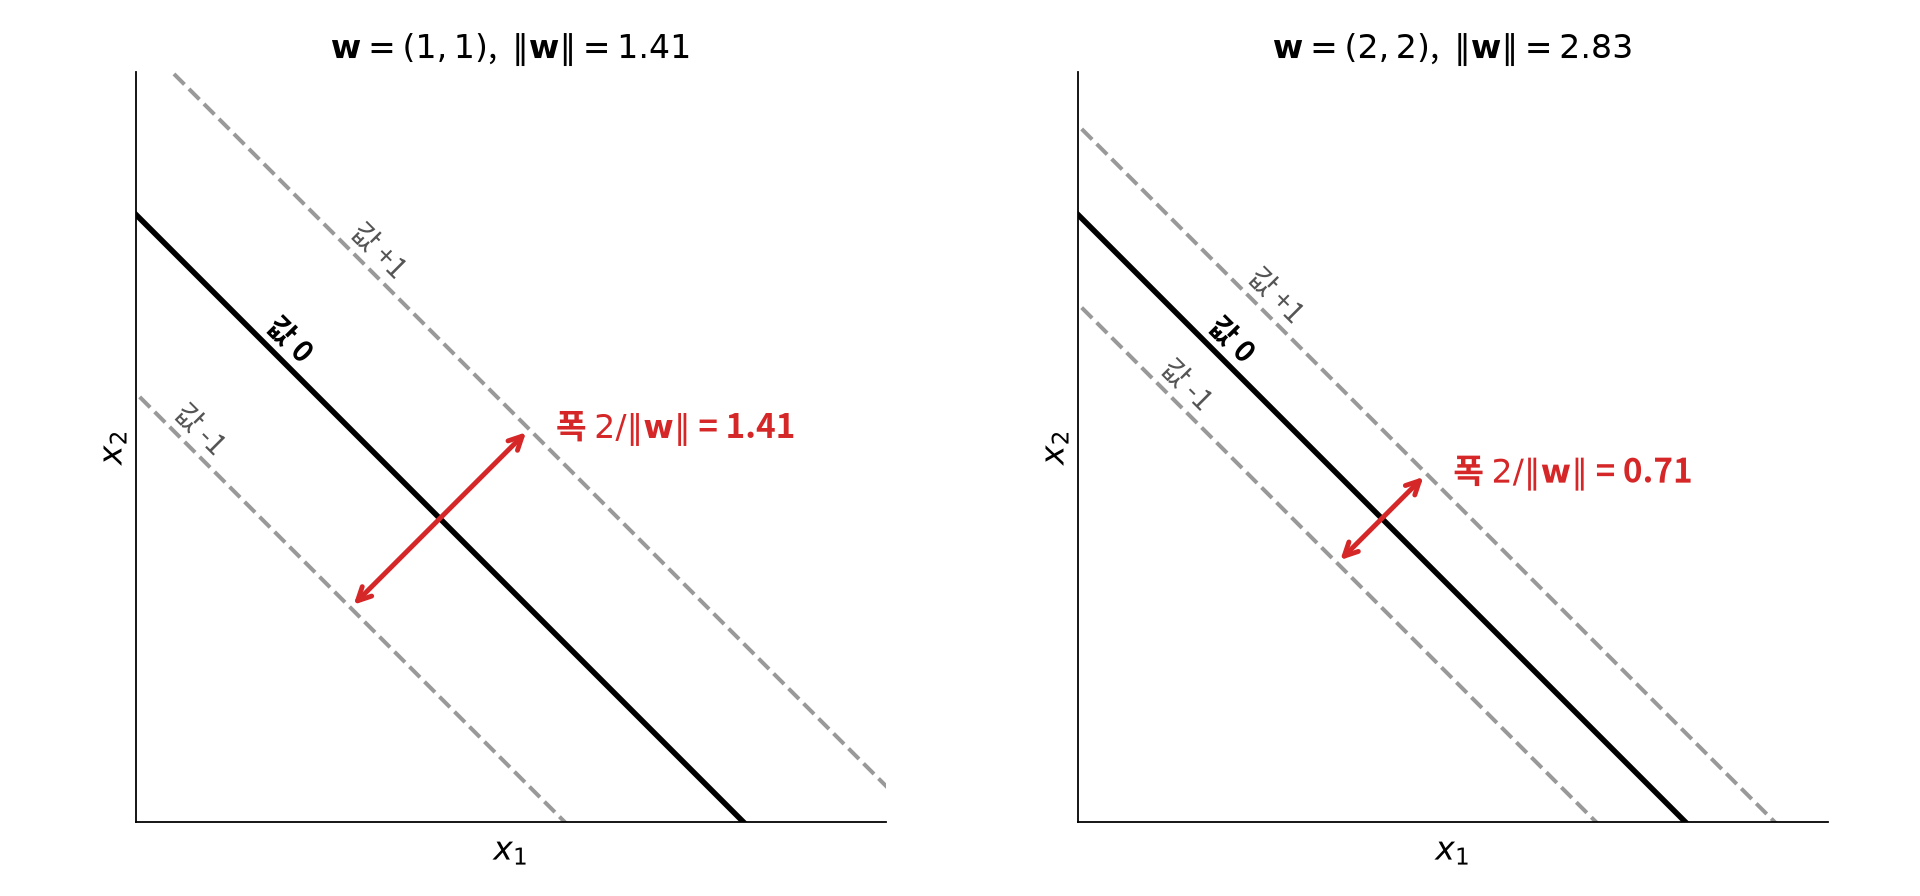
\includegraphics[width=0.74\linewidth]{sv_width.png}\par\vskip0.2em
{\large 경계에서 값 $+1$ 선까지 $1/\lVert\mathbf{w}\rVert$, 값 $-1$ 선까지 $1/\lVert\mathbf{w}\rVert$ \;$\Rightarrow$\; 폭 \kb{$2/\lVert\mathbf{w}\rVert$}}\\[0.3em]
{\large $\lVert\mathbf{w}\rVert$ 가 \kq{작을수록} 길이 넓다}
\vfill
\note{반대쪽도 똑같습니다. w 반대 방향으로 1 나누기 w의 길이만큼 걸으면 값이 마이너스 1입니다. 그래서 값 마이너스 1인 선과 플러스 1인 선 사이, 길의 폭은 2 나누기 w의 길이입니다. 왼쪽은 w가 1, 1, 길이 1.41이라 폭이 1.41입니다. 오른쪽처럼 w를 2, 2로 키우면 같은 경계인데 값이 두 배 빨리 오르니까 플러스 마이너스 1 선이 경계에 바짝 붙어서 폭이 0.71로 줄어듭니다. 거꾸로 말하면 w의 길이가 작을수록 플러스 마이너스 1 선이 멀리 떨어지고 길이 넓어집니다. 그런데 모든 점이 가장자리 바깥에 있어야 한다는 조건을 걸면, w를 아무리 작게 하고 싶어도 가장 가까운 점이 가장자리에 걸려서 멈춥니다. 그 멈춘 곳이 가장 넓은 길입니다. 다음 쪽이 이것을 식으로 쓴 것입니다.}
\end{frame}

% --- 식
\begin{frame}{길을 식으로}
\markpage{form}
\vfill
\centering
{\Large 경계 \quad $\mathbf{w}\cdot\mathbf{x} + b = 0$ \qquad 가장자리 \quad $\mathbf{w}\cdot\mathbf{x} + b = \pm 1$}\\[0.6em]
{\LARGE\[ \min_{\mathbf{w},\,b}\ \frac{1}{2}\lVert\mathbf{w}\rVert^2 \quad \text{subject to} \quad y_i(\mathbf{w}\cdot\mathbf{x}_i + b) \ge 1 \;\; (\text{all } i) \]}\vskip0.2em
\renewcommand{\arraystretch}{1.25}
{\normalsize\begin{tabular}{ll}
$y_i = +1$ (빨강), $-1$ (파랑) & 모든 점이 자기 쪽 가장자리 바깥에 있어야 한다\\
마진 $= 2 / \lVert\mathbf{w}\rVert$ & $\lVert\mathbf{w}\rVert$ 를 줄이면 길이 넓어진다\\
이 데이터 & $\mathbf{w} = \tfrac{4}{9}(-1, 1)$, \; $b = -\tfrac{1}{9}$ \; $\to$ \; $2/\lVert\mathbf{w}\rVert = \tfrac{9}{2\sqrt2} = 3.18$
\end{tabular}}
\vfill
\note{길을 식으로 쓰면 이렇습니다. 경계는 w 점곱 x 더하기 b가 0인 직선, 길 가장자리는 이 값이 플러스 1과 마이너스 1인 직선입니다. 빨강의 라벨을 플러스 1, 파랑을 마이너스 1이라고 하면, 모든 점이 자기 쪽 가장자리 바깥에 있다는 조건은 y 곱하기 w x 더하기 b가 1 이상이라는 한 줄로 쓸 수 있습니다. 두 가장자리 사이의 거리를 계산하면 2 나누기 w의 길이가 나옵니다. 그래서 길을 가장 넓게 하는 것은 w의 길이를 가장 작게 하는 것과 같습니다. 이 데이터에서는 w가 9분의 4 곱하기 마이너스 1, 1이고 b는 마이너스 9분의 1, 마진은 3.18입니다.}
\end{frame}

% --- 학습 0: 숫자 3개 찾기
\begin{frame}{직선 찾기 = 숫자 3개 $(w_1, w_2, b)$ 찾기}
\vfill
\centering
{\LARGE 경계 \quad $w_1 x_1 + w_2 x_2 + b = 0$}\\[1em]
{\large 점 20개는 주어져 있다 $\to$ 정할 것은 \kb{$w_1$, $w_2$, $b$} 세 숫자뿐}\\[1em]
\renewcommand{\arraystretch}{1.4}
{\large\begin{tabular}{rl}
\textbf{1.} & $(w_1, w_2, b) = (0, 0, 0)$ 에서 출발\\
\textbf{2.} & 점 20개를 넣어 보고 \kq{틀린 · 아슬아슬한 점}을 찾는다\\
\textbf{3.} & 그 점이 맞는 쪽으로 가도록 세 숫자를 \textbf{조금} 고친다\\
\textbf{4.} & 2--3 을 반복 (로지스틱회귀의 경사하강법과 같다)
\end{tabular}}
\vfill
\note{그래서 이 직선을 어떻게 찾을까요. 경계는 w1 x1 더하기 w2 x2 더하기 b가 0인 직선입니다. 점 20개는 이미 주어져 있으니 우리가 정할 것은 w1, w2, b 세 숫자뿐입니다. 이 세 숫자를 찾는 것이 학습입니다. 방법은 로지스틱회귀 때와 같습니다. 0, 0, 0에서 출발해서 점 20개를 넣어 보고, 틀렸거나 아슬아슬한 점을 찾아 그 점이 맞는 쪽으로 가도록 세 숫자를 조금 고칩니다. 이것을 수천 번 반복합니다. 다음 쪽에서 무엇을 아슬아슬하다고 하는지, 얼마나 고치는지 보겠습니다.}
\end{frame}

% --- 학습 1: 여유와 한 걸음
\begin{frame}{학습 \textcircled{1}: 여유가 1 보다 작은 점만 민다}
\markpage{train}
\vfill
\centering
{\Large 점마다 \kb{여유} $= y_i(\mathbf{w}\cdot\mathbf{x}_i + b)$}\\[0.3em]
{\large 점수에 색 ($\pm 1$) 을 곱한 값: 자기 쪽으로 얼마나 깊이 들어와 있나}\\[0.8em]
\renewcommand{\arraystretch}{1.3}
{\large\begin{tabular}{l|l}
여유 $\ge 1$ & 자기 쪽 가장자리 바깥 $\to$ \textbf{가만히}\\
여유 $< 1$ & 길 안 · 반대편 $\to$ \kq{경계를 민다}
\end{tabular}}\\[0.8em]
{\large 한 걸음 ($\eta$ = 학습률)}\\[0.3em]
{\large \textbf{1.} $\mathbf{w} \leftarrow \mathbf{w} - \eta\,\mathbf{w}$ \quad ($\lVert\mathbf{w}\rVert$ 가 줄어 \kb{길이 넓어진다})}\\[0.2em]
{\large \textbf{2.} 여유 $< 1$ 인 점마다 \; $\mathbf{w} \leftarrow \mathbf{w} + \eta\, y_i \mathbf{x}_i$, \; $b \leftarrow b + \eta\, y_i$}
\vfill
\note{이제 SVM이 실제로 어떻게 학습하는지 봅시다. 점마다 여유라는 값을 잽니다. 점수 w x 더하기 b에 그 점의 색, 빨강이면 플러스 1, 파랑이면 마이너스 1을 곱한 값입니다. 빨간 점이 빨강 쪽 깊숙이 있으면 점수가 큰 양수라 여유가 크고, 파란 점이 파랑 쪽 깊숙이 있으면 점수가 큰 음수인데 마이너스 1을 곱하니 역시 여유가 큽니다. 여유가 1 이상이면 자기 쪽 가장자리 바깥이라 아무 일도 하지 않습니다. 여유가 1보다 작으면 길 안에 들어와 있거나 반대편에 있다는 뜻이고, 이 점이 경계를 밉니다. 한 걸음은 두 가지입니다. 첫째, w를 조금 줄입니다. w의 길이가 줄면 앞에서 본 것처럼 길이 넓어집니다. 둘째, 여유가 1보다 작은 점마다 w에 그 점을 색 부호를 붙여 조금 더하고 b도 조금 움직입니다. 그러면 그 점의 점수가 자기 쪽으로 커져서 길 밖으로 밀려납니다. 로지스틱회귀에서 했던 경사하강법과 같은 반복입니다. 손실을 힌지 손실이라고 부르는데, 이름은 몰라도 됩니다. 실습에서는 학습률 0.02를 걸음 수의 제곱근으로 나눠 씁니다.}
\end{frame}

% --- 학습 1.5: 숫자로 따라가기
\begin{frame}{학습을 숫자로 따라가 보면}
\vfill
\centering
\renewcommand{\arraystretch}{1.25}
{\large\begin{tabular}{r|rrr|r|l}
걸음 & $w_1$ & $w_2$ & $b$ & 폭 $2/\lVert\mathbf{w}\rVert$ & 미는 점\\ \hline
1 & 0 & 0 & 0 & -- & \kq{20개 모두} (여유 0)\\
2 & $-0.88$ & $0.78$ & 0 & 1.69 & 없음\\
100 & $-0.62$ & $0.55$ & 0 & 2.41 & 없음 (길만 넓어진다)\\
176 & $-0.54$ & $0.48$ & 0 & 2.74 & (3.5, 6) 이 처음 닿음\\
278 & $-0.46$ & $0.45$ & 0 & 3.12 & (5, 3) 이 처음 닿음\\
20,000 & $-0.45$ & $0.44$ & $-0.10$ & \kb{3.18} & 서포트 벡터 3개가 번갈아\\ \hline
SVM 답 & $-0.44$ & $0.44$ & $-0.11$ & 3.18 &
\end{tabular}}\\[0.8em]
{\normalsize 1걸음: $\mathbf{w} = 0.02 \times \sum_i y_i \mathbf{x}_i = 0.02 \times (-44.1,\ 39.2) = (-0.88,\ 0.78)$}
\vfill
\note{실제로 점 20개로 돌린 숫자입니다. 1걸음에서는 w가 0이라 모든 점의 점수가 0, 여유도 0이라서 20개가 모두 밉니다. 빨간 점은 자기 좌표를 더하고 파란 점은 빼서, 모두 합하면 마이너스 44.1, 39.2이고 학습률 0.02를 곱하면 w가 마이너스 0.88, 0.78이 됩니다. 이미 대충 맞는 방향의 선입니다. 2걸음부터는 길 안에 점이 하나도 없어서 w를 줄이기만 합니다. w가 작아지니 폭이 1.69, 2.41로 넓어집니다. 176걸음에서 넓어진 길이 빨간 점 3.5, 6에 처음 닿고, 이 점이 밀기 시작합니다. 278걸음에 파란 점 5, 3도 닿습니다. 2만 걸음이면 w가 마이너스 0.45, 0.44, b가 마이너스 0.10, 폭 3.18로 sklearn이 낸 SVM 답과 소수 둘째 자리까지 거의 같습니다.}
\end{frame}

% --- 학습 2: 걸음별
\begin{frame}{학습 \textcircled{2}: 반복하면 미는 점이 3개만 남는다}
\vfill
\centering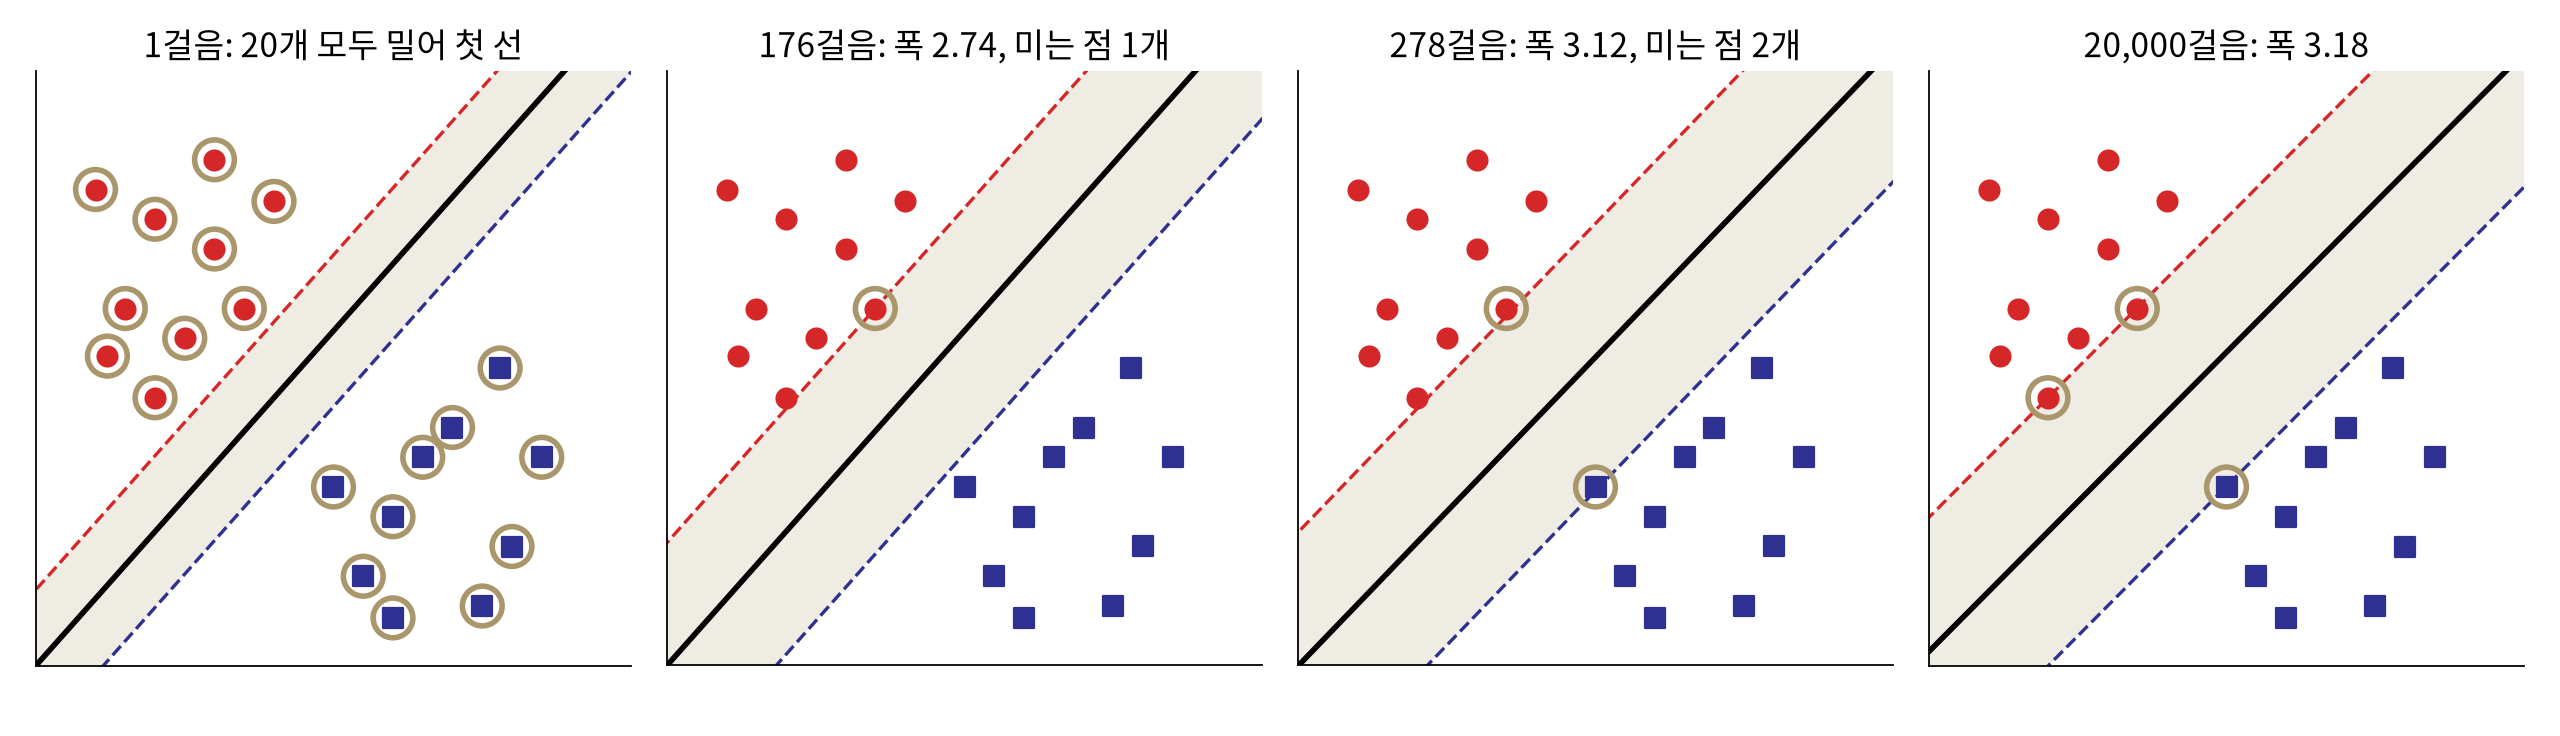
\includegraphics[width=\linewidth]{sv_train4.png}\par\vskip0.3em
{\large 처음 밀기 시작한 걸음: \kb{(3.5, 6)} 176 \;·\; \kb{(5, 3)} 278 \;·\; \kb{(2, 4.5)} 7,567}\\[0.2em]
{\large 나머지 17개는 1걸음 뒤로 \kq{한 번도} 안 밀었다}
\vfill
\note{점 20개로 실제로 2만 걸음 돌린 결과입니다. 처음엔 w가 0이라 모든 점의 여유가 0, 20개가 전부 밀어서 첫 선이 생깁니다. 그다음부터는 길 안에 점이 없으니 첫째 일, w 줄이기만 합니다. 길이 점점 넓어집니다. 176걸음째 넓어진 길이 빨간 점 3.5, 6에 닿고, 이 점이 밀기 시작합니다. 278걸음째 파란 점 5, 3도 닿습니다. 7567걸음째 빨간 점 2, 4.5가 닿습니다. 이 셋이 번갈아 밀면서 길이 더 넓어지지 못하게 붙잡고, 2만 걸음에서 폭 3.18, 앞에서 본 답에 도착합니다. 첫 걸음 뒤로 나머지 17개 점은 한 번도 밀지 않았습니다.}
\end{frame}

% --- 학습 3: 가려내기
\begin{frame}{학습 \textcircled{3}: 끝나고 여유를 재면 서포트 벡터가 보인다}
\vfill
\centering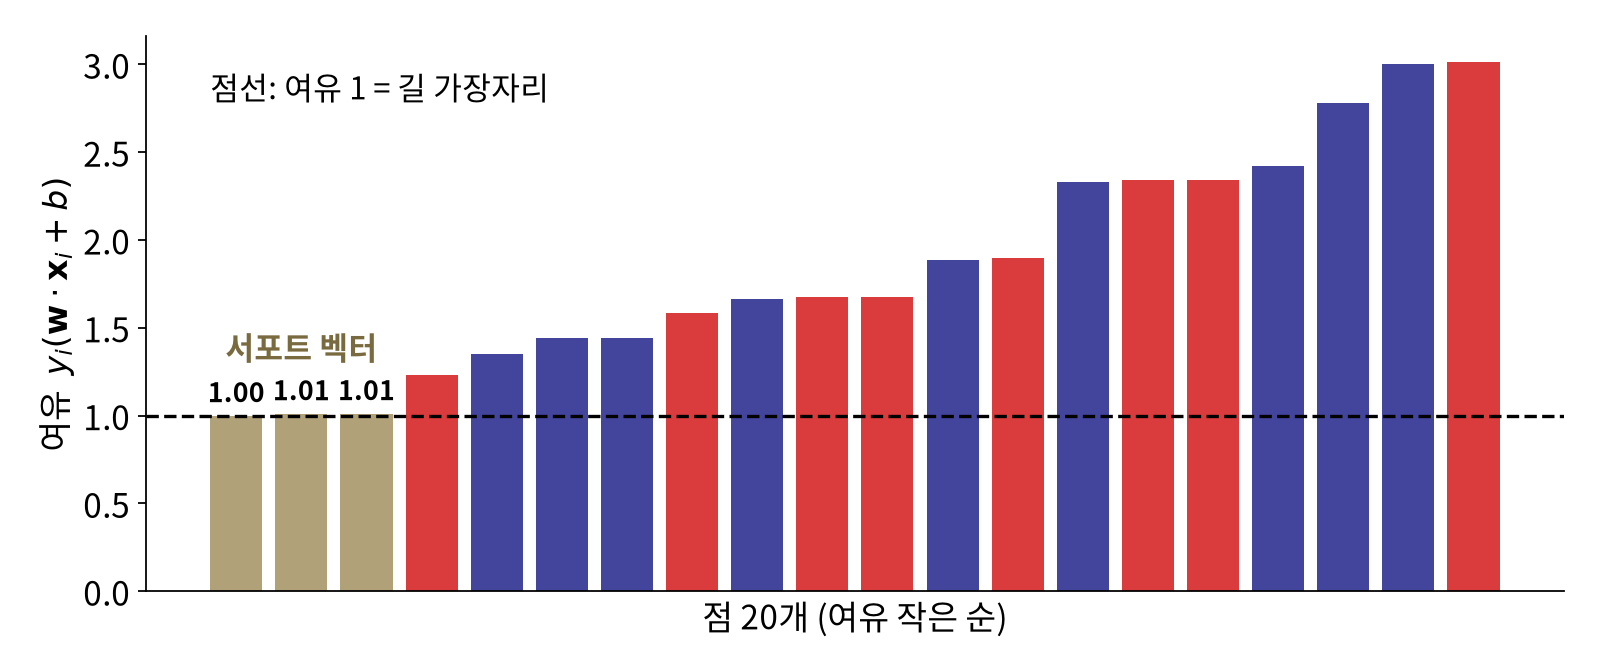
\includegraphics[width=0.78\linewidth]{sv_slack_bars.png}\par\vskip0.2em
{\large 여유 $= 1$ (가장자리 위) = \kb{서포트 벡터} \quad 나머지는 모두 $1.2$ 이상}\\[0.2em]
{\small sklearn \texttt{SVC} 는 다른 풀이법 (SMO) 으로 같은 답 $\to$ \texttt{support\_vectors\_} 에 3개}
\vfill
\note{학습이 끝난 뒤 점 20개의 여유를 작은 순서로 막대로 그렸습니다. 세 점이 1.00, 1.01, 1.01로 점선, 즉 길 가장자리 위에 있습니다. 이 셋이 서포트 벡터입니다. 나머지 17개는 모두 1.2 이상, 가장자리 바깥에 여유 있게 있습니다. 그러니 서포트 벡터를 미리 고르는 게 아니라, 학습하면서 끝까지 미는 점이 저절로 서포트 벡터가 되고, 학습이 끝난 뒤 여유가 1인 점을 보면 가려낼 수 있습니다. 실무에서 쓰는 sklearn의 SVC는 이런 경사하강 대신 SMO라는 다른 풀이법을 쓰지만 같은 답을 내고, support vectors라는 속성에 이 3개를 담아 줍니다.}
\end{frame}

% --- 서포트 벡터만
\begin{frame}{길 가장자리의 점 몇 개만 선을 정한다}
\vfill
\centering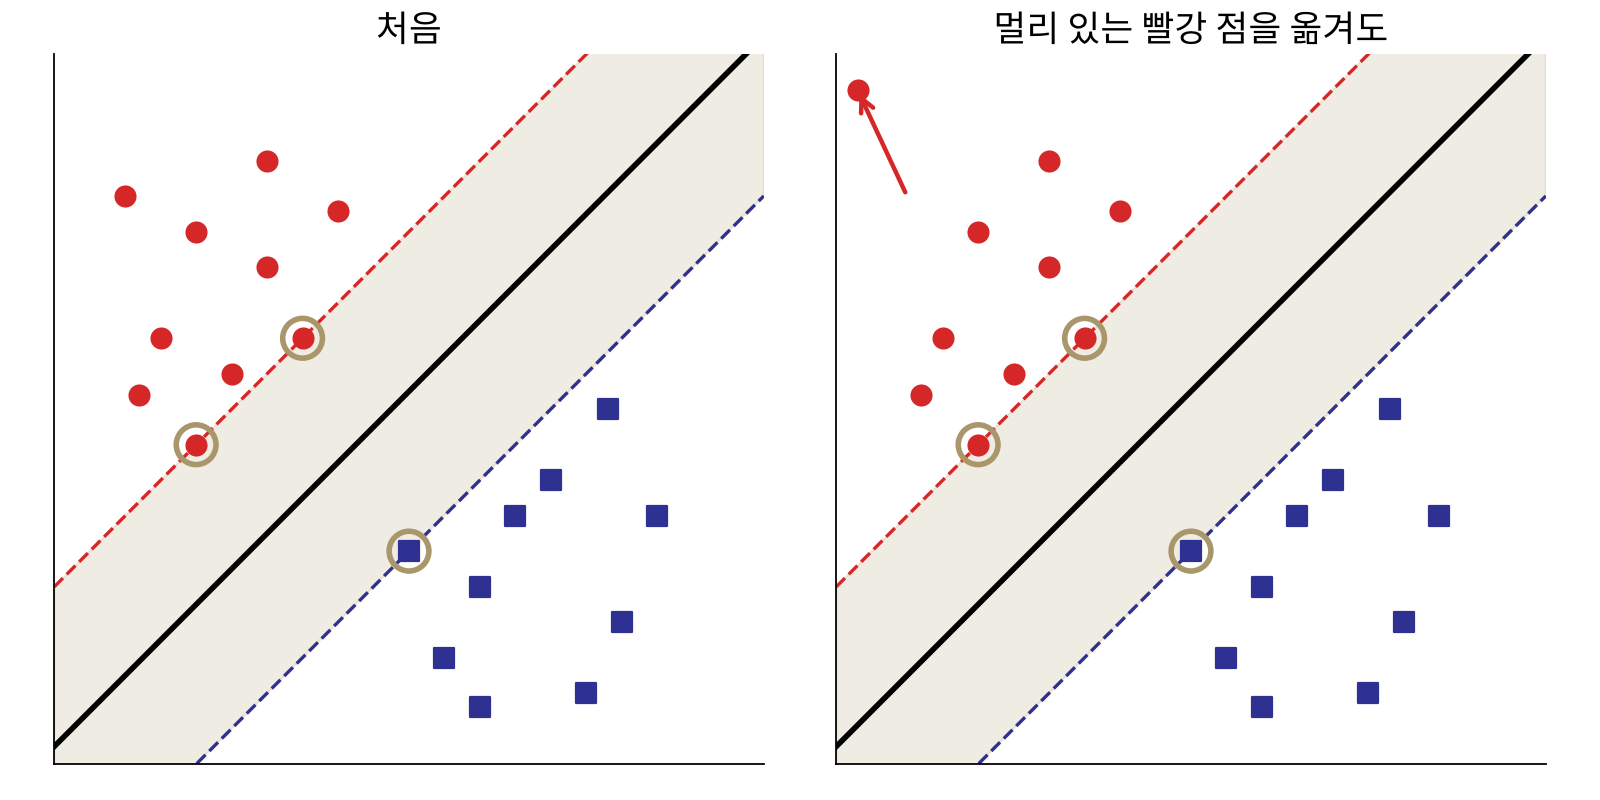
\includegraphics[width=0.66\linewidth]{sv_move.png}\par\vskip0.2em
{\large 서포트 벡터 \kb{3개}: \; $(3.5, 6.0)$, $(2.0, 4.5)$ 빨강 \quad $(5.0, 3.0)$ 파랑}\\[0.2em]
{\large 멀리 있는 점은 옮겨도 경계가 \kq{그대로}}
\vfill
\note{이 경계는 20개 점 중 단 3개, 서포트 벡터가 정합니다. 빨강 둘, 파랑 하나입니다. 길 가장자리에서 멀리 떨어진 점은 경계에 아무 영향이 없습니다. 오른쪽 그림에서 왼쪽 위의 빨간 점 하나를 더 멀리 옮겼는데, 경계와 길은 그대로입니다. 반대로 서포트 벡터 하나를 옮기면 경계가 바뀝니다. 로지스틱회귀는 모든 점이 조금씩 경계에 영향을 주는 것과 대조적입니다.}
\end{frame}

% --- 서포트 벡터가 3개만 남는 과정: 방향 돌리기
\begin{frame}{어떻게 3개만 남나 \textcircled{1}: 방향을 정하고 길을 넓힌다}
\vfill
\centering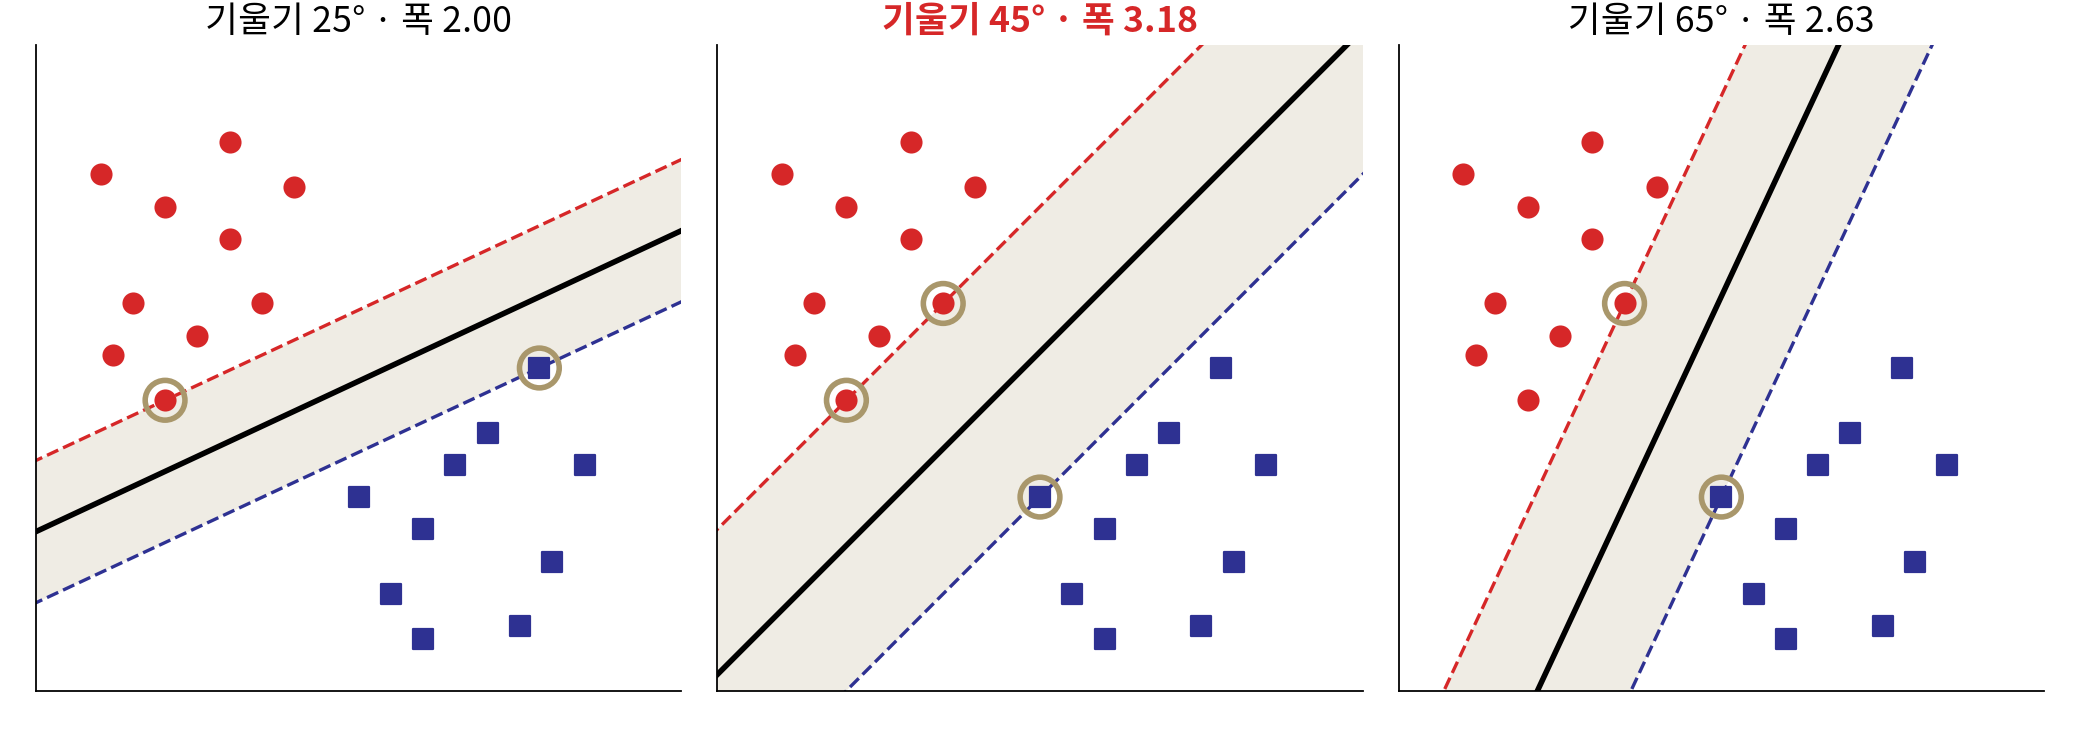
\includegraphics[width=0.96\linewidth]{sv_sweep3.png}\par\vskip0.3em
{\large 길을 넓히다 보면 \kb{가장 가까운 빨강 · 파랑}에 닿아 멈춘다}
\vfill
\note{20개 점 중에서 왜 딱 3개만 남는지, 계산 과정을 단계별로 봅시다. 먼저 선의 방향을 하나 정합니다. 왼쪽은 기울기 25도입니다. 이 방향 그대로 길을 양쪽으로 넓혀 갑니다. 그러다 빨간 점 하나, 파란 점 하나에 닿으면 더 못 넓힙니다. 노란 동그라미가 닿은 점입니다. 폭은 2.00입니다. 이때 길을 정한 건 이 두 점뿐이고, 나머지 18개는 아무 역할이 없습니다. 기울기 45도로 바꾸면 폭이 3.18, 65도면 2.63입니다. 방향마다 닿는 점이 바뀝니다.}
\end{frame}

\begin{frame}{어떻게 3개만 남나 \textcircled{2}: 방향을 돌려 가며 폭을 잰다}
\vfill
\centering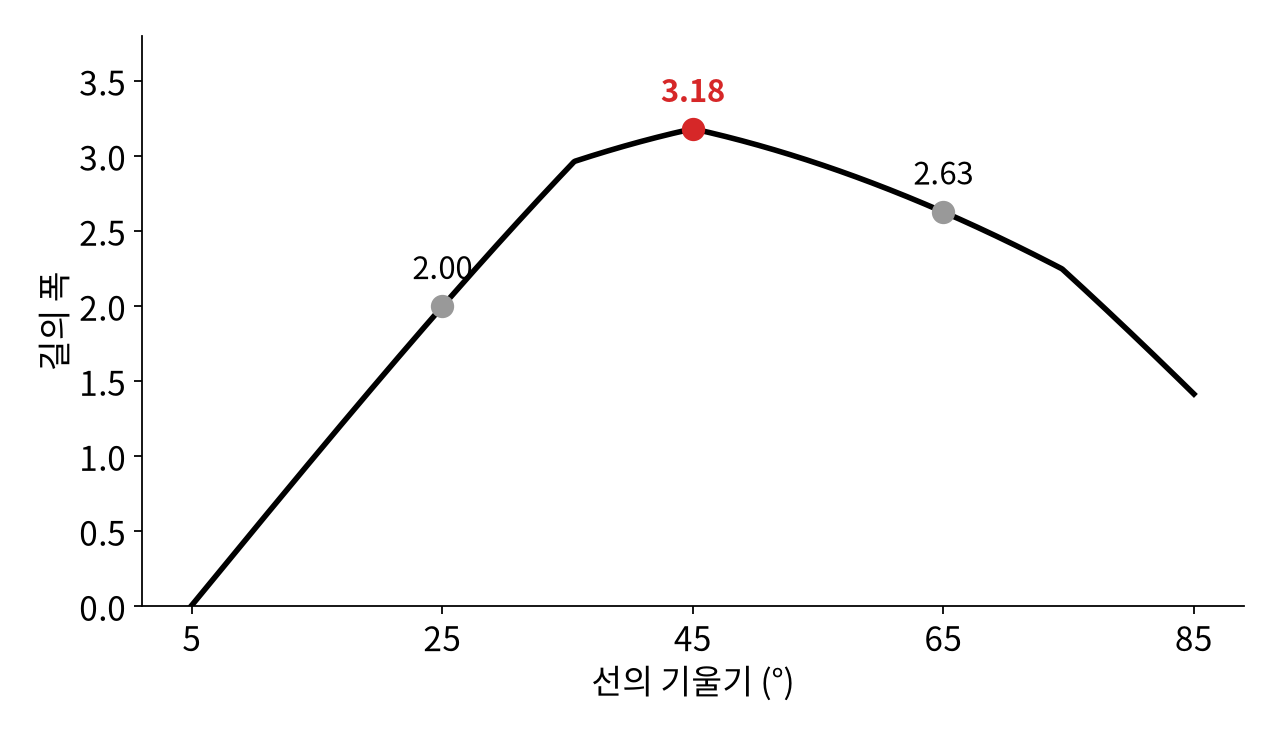
\includegraphics[width=0.64\linewidth]{sv_sweep_curve.png}\par\vskip0.2em
{\large 가장 넓은 곳: 기울기 \kb{45°}, 폭 \kb{3.18} \;$\to$\; 점 \kq{3개}가 동시에 닿는다}
\vfill
\note{이번엔 기울기를 5도부터 85도까지 조금씩 돌리면서 폭을 재 그래프로 그렸습니다. 25도에서 2.00, 45도에서 3.18, 65도에서 2.63입니다. 꼭대기가 45도, 폭 3.18이고 앞에서 본 SVM의 마진과 같습니다. 꼭대기에서는 빨간 점 두 개와 파란 점 하나, 3개가 동시에 가장자리에 닿습니다. 왼쪽으로 조금 돌리면 빨간 점 하나가, 오른쪽으로 돌리면 다른 빨간 점이 길을 파고들어서 폭이 줄어듭니다. 그래서 더 못 돌립니다. 평면의 길은 방향, 위치, 폭 세 가지로 정해지니, 보통 점 3개가 닿으면 꼼짝 못 하게 됩니다. 실제 라이브러리는 이렇게 각도를 하나하나 돌리지 않고 앞 쪽의 최소화 문제를 바로 풀지만, 답은 같습니다.}
\end{frame}

\begin{frame}{어떻게 3개만 남나 \textcircled{3}: 닿지 않은 17개는 빼도 같은 길}
\vfill
\centering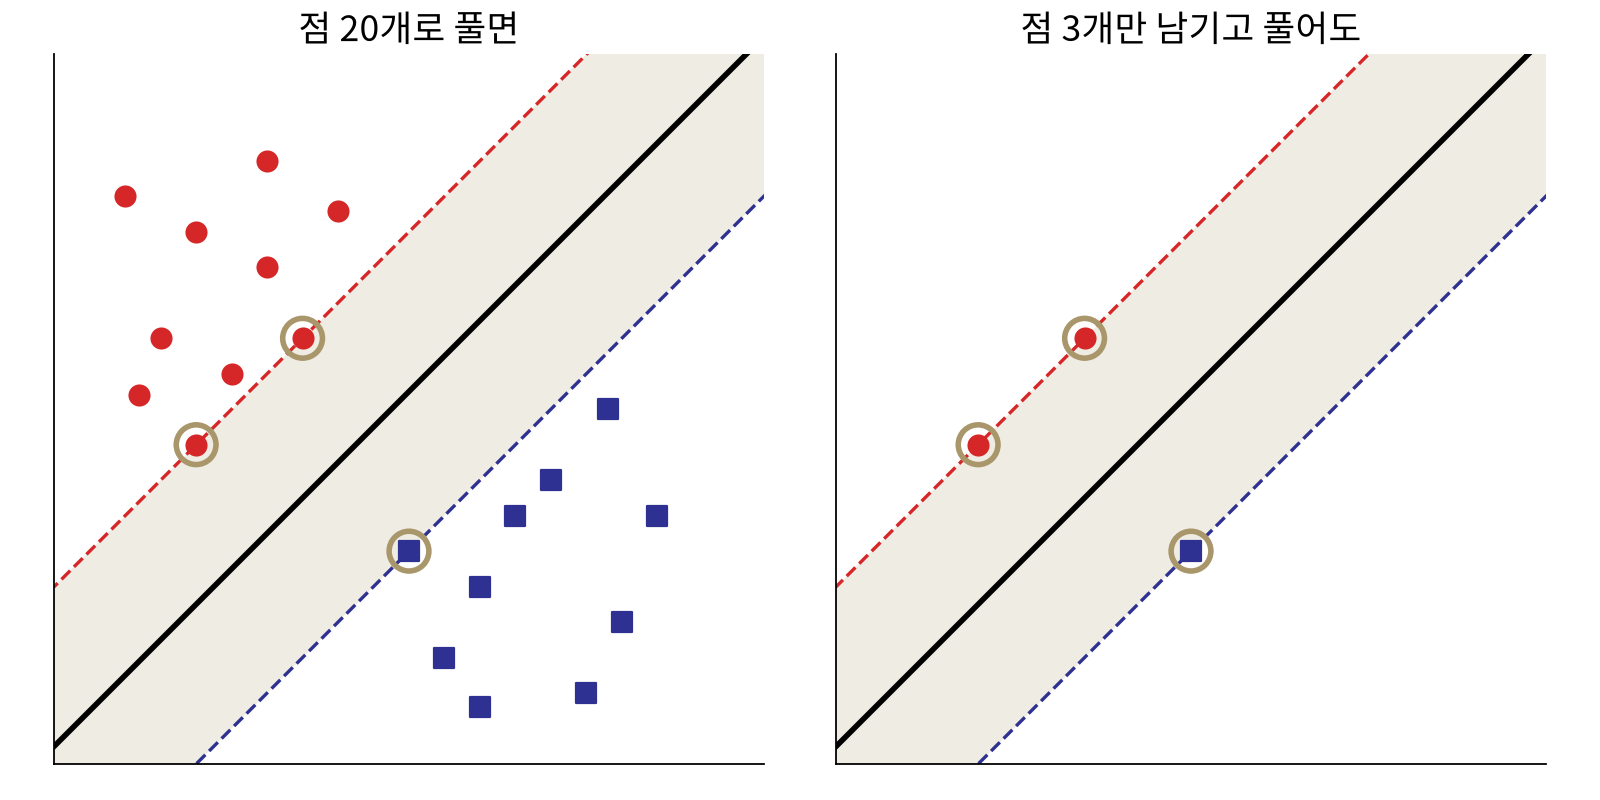
\includegraphics[width=0.66\linewidth]{sv_only3.png}\par\vskip0.2em
{\large 꼭대기에서 닿은 점 3개 = \kb{서포트 벡터}}
\vfill
\note{확인해 봅시다. 왼쪽은 점 20개로 푼 SVM, 오른쪽은 닿은 점 3개만 남기고 나머지 17개를 지운 뒤 다시 푼 SVM입니다. 경계도, 길도, 폭 3.18도 똑같습니다. 꼭대기에서 길을 붙잡고 있던 점 3개, 이것이 서포트 벡터입니다. 나머지 점은 길 바깥에 여유 있게 떨어져 있어서 지워도, 앞에서 본 것처럼 옮겨도 답이 바뀌지 않습니다.}
\end{frame}

\section{소프트 마진}
% --- 소프트 마진
\begin{frame}{완벽히 나뉘지 않으면: 소프트 마진}
\markpage{soft}
\vfill
\centering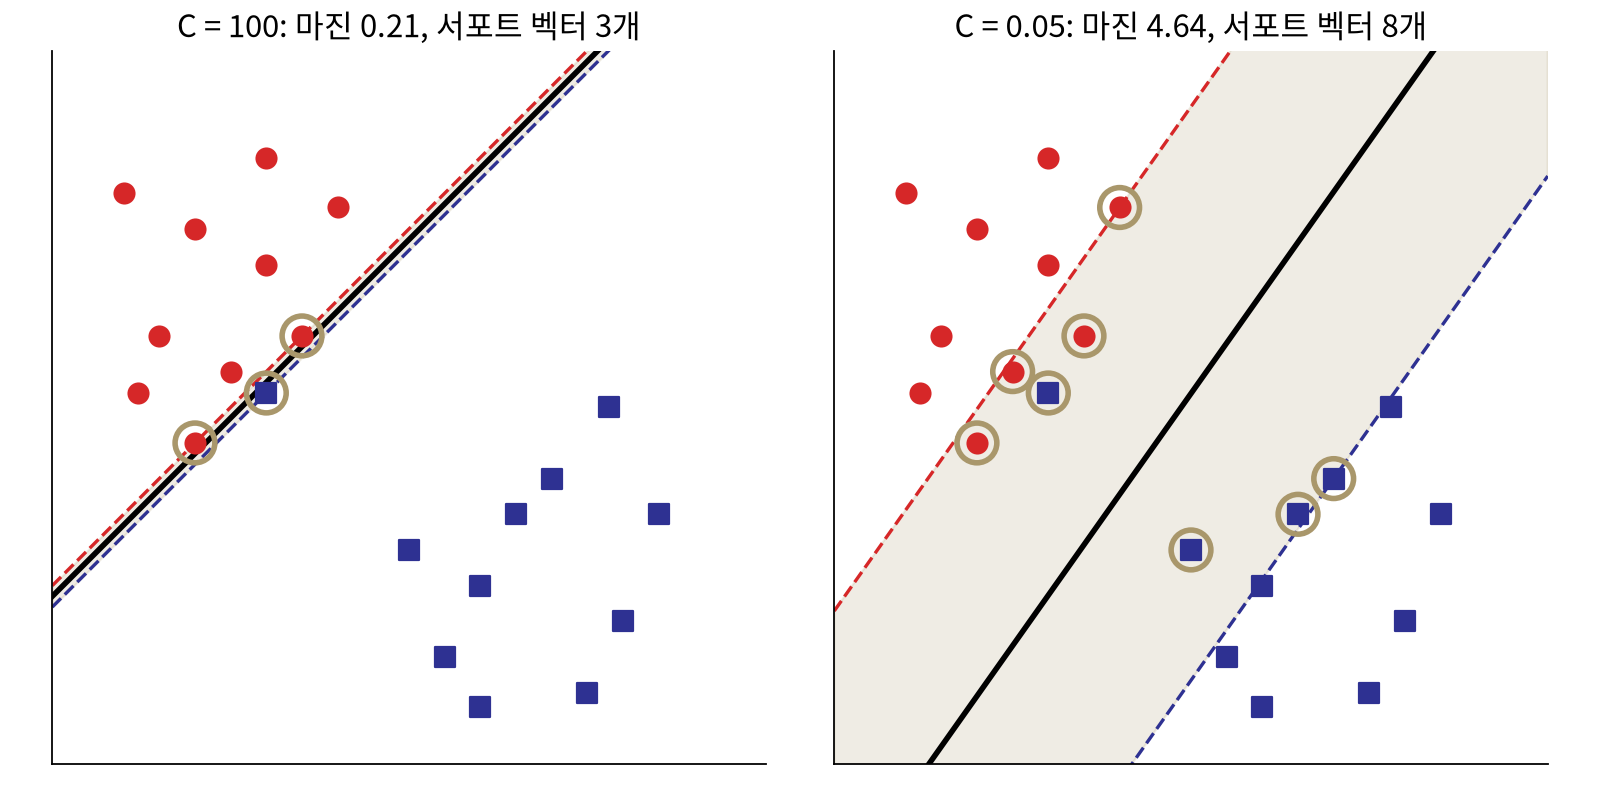
\includegraphics[width=0.53\linewidth]{sv_soft.png}\par\vskip0.1em
{\large\[ \min\ \frac{1}{2}\lVert\mathbf{w}\rVert^2 + \textcolor{ksared}{C}\sum_i \xi_i \qquad \xi_i: \text{가장자리를 넘어간 만큼의 벌점} \]}
{\large $C$ 크면 \kq{안 틀리려고} 좁은 길 (0.21) \quad $C$ 작으면 이상치는 \kb{포기}, 넓은 길 (4.64)}
\vfill
\note{실제 데이터는 이렇게 깔끔하게 나뉘지 않습니다. 빨강 무리 안에 파란 점 하나가 들어왔다고 해 봅시다. 측정 실수일 수도 있습니다. 이러면 길 안에 점이 하나도 없어야 한다는 조건을 지킬 수 없습니다. 그래서 가장자리를 넘어가는 것을 허락하되, 넘어간 만큼 벌점 크사이를 줍니다. C는 그 벌점의 무게입니다. C가 100으로 크면 하나도 틀리지 않으려고 이상치를 피해 가느라 길 폭이 0.21로 아주 좁아집니다. C가 0.05로 작으면 이상치 하나는 틀리기로 하고 4.64짜리 넓은 길을 냅니다. C가 크면 과대적합, 작으면 과소적합 쪽입니다. 그래서 C도 교차 검증으로 고릅니다.}
\end{frame}

\section{커널}
% --- 원 모양 데이터
\begin{frame}{직선으로 못 가르면: 높이를 준다}
\markpage{lift}
\vfill
\centering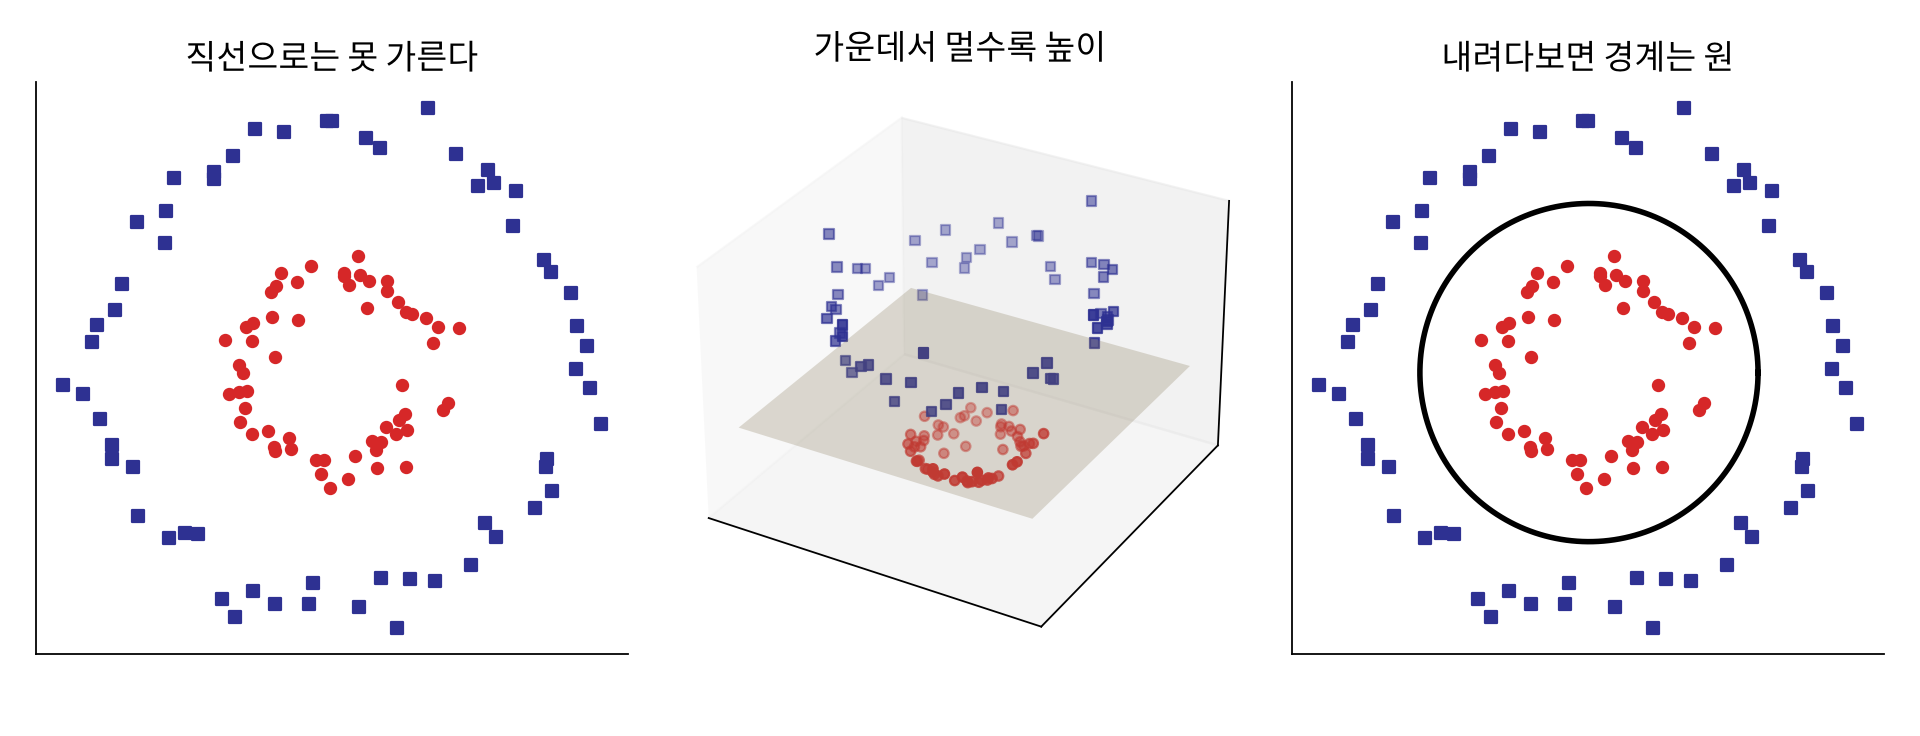
\includegraphics[width=0.94\linewidth]{sv_lift.png}\par\vskip0.2em
{\large 특징 하나를 더한다: \; $(x_1,\ x_2) \;\to\; (x_1,\ x_2,\ \textcolor{ksablue}{x_1^2 + x_2^2})$ \quad $\to$ \quad 평면 하나로 갈라진다}
\vfill
\note{이번에는 빨간 점이 가운데, 파란 점이 바깥을 둘러싼 데이터입니다. 어떤 직선을 그어도 가를 수 없습니다. 그런데 각 점에 높이를 하나 더 줘 봅시다. 가운데서 떨어진 거리의 제곱, x1 제곱 더하기 x2 제곱입니다. 그러면 가운데 빨간 점은 낮게, 바깥 파란 점은 높게 떠서, 가운데 그림처럼 수평한 평면 하나로 깔끔하게 갈라집니다. 이 평면을 원래 평면에서 내려다보면 오른쪽처럼 원이 됩니다. 높은 차원에서 직선으로 가르면, 원래 차원에서는 휘어진 경계가 됩니다. 선형회귀에 x 제곱 특징을 넣은 것과 같은 아이디어입니다.}
\end{frame}

% --- 커널 트릭
\begin{frame}{커널 트릭: 옮기지 않고 계산만}
\markpage{kernel}
\vfill
\centering
{\large SVM 의 계산에는 점끼리의 \textbf{점곱} $\mathbf{x}\cdot\mathbf{x}'$ 만 나온다 $\to$ 점곱 대신 \kb{커널} $K(\mathbf{x},\mathbf{x}')$}\vskip0.3em
{\normalsize 경계 식도 점곱으로: \; $\mathbf{w}\cdot\mathbf{x} + b = b + \sum_i \alpha_i\, \mathbf{x}\cdot\mathbf{x}^{(i)}$ \quad ($\alpha_i \ne 0$ 인 점 = \kb{서포트 벡터})}\par\vskip0.05em
{\tiny\color{gray} Goodfellow, Bengio, Courville, \textit{Deep Learning} (2016), 5.7.2 식 (5.82)}\vskip0.2em
{\Large\[ \phi(\mathbf{x}) = (x_1^2,\ \sqrt2\,x_1x_2,\ x_2^2) \quad\Rightarrow\quad \phi(\mathbf{x})\cdot\phi(\mathbf{x}') = (\mathbf{x}\cdot\mathbf{x}')^2 \]}\vskip0.2em
{\large $\mathbf{x} = (1, 2)$, $\mathbf{x}' = (3, 1)$: \quad $(1, 2\sqrt2, 4)\cdot(9, 3\sqrt2, 1) = 9 + 12 + 4 = 25 = (3 + 2)^2$}\\[0.6em]
{\large RBF 커널 \; $K(\mathbf{x},\mathbf{x}') = \exp\!\big(-\gamma\lVert\mathbf{x}-\mathbf{x}'\rVert^2\big)$ \; = 무한 차원으로 옮긴 것과 같다}
\vfill
\note{높은 차원으로 옮기면 특징이 많아져 계산이 무거워집니다. 그런데 SVM을 풀 때는 점 자체가 아니라 점끼리의 점곱만 필요하다는 게 알려져 있습니다. 굿펠로의 딥러닝 교과서 5.7.2절처럼, 경계 식 w 점곱 x 더하기 b 자체를 학습 데이터와의 점곱에 계수 알파를 곱해 더한 꼴로 다시 쓸 수 있습니다. 학습이 끝나면 알파는 대부분 0이고, 0이 아닌 점이 서포트 벡터, 앞에서 본 끝까지 경계를 민 점들입니다. 그래서 옮긴 뒤의 점곱을 옮기지 않고 바로 계산하는 함수, 커널을 씁니다. 예를 들어 2차원 점을 x1 제곱, 루트2 x1 x2, x2 제곱인 3차원으로 옮기면, 옮긴 뒤의 점곱은 원래 점곱의 제곱과 정확히 같습니다. (1, 2)와 (3, 1)이면 옮겨서 계산해도 25, 원래 점곱 5를 제곱해도 25입니다. 이렇게 옮기지 않고 계산만 하는 요령이 커널 트릭입니다. 가장 많이 쓰는 RBF 커널은 무한 차원으로 옮긴 것과 같은 효과를 내는데도 계산은 거리 하나면 됩니다.}
\end{frame}

% --- gamma
\begin{frame}{RBF 커널의 $\gamma$: 얼마나 구불구불하게}
\vfill
\centering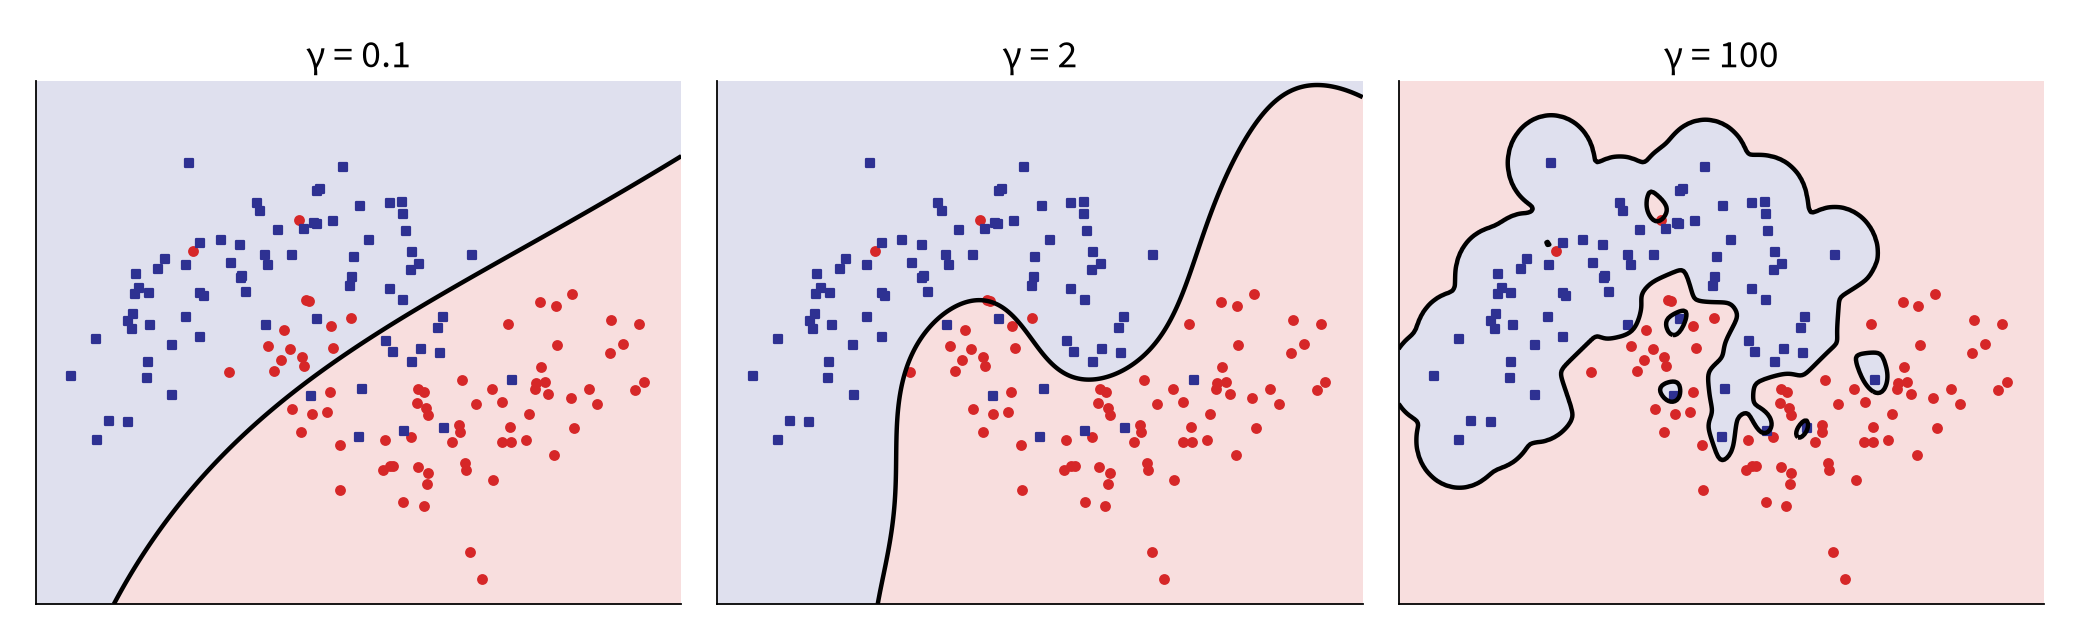
\includegraphics[width=0.92\linewidth]{sv_gamma.png}\par\vskip0.2em
{\large $\gamma$ 작으면 거의 직선 (과소적합) \quad $\gamma$ 크면 점마다 섬 (\kq{과대적합}) \quad $\to$ $C$, $\gamma$ 는 교차 검증으로}
\vfill
\note{RBF 커널의 감마는 점 하나의 영향이 얼마나 멀리까지 미치는지를 정합니다. 감마가 0.1로 작으면 영향이 넓게 퍼져서 경계가 거의 직선입니다. 반달 모양을 못 따라가는 과소적합입니다. 감마가 2면 반달을 따라 적당히 휘어집니다. 감마가 100이면 점 하나하나의 영향이 아주 좁아서 점마다 섬이 생깁니다. 학습 데이터를 외운 과대적합입니다. 그래서 SVM을 쓸 때는 C와 감마 두 숫자를 교차 검증으로 함께 고릅니다. 실습에서 직접 해 봅니다.}
\end{frame}

\section{연습}
% --- 문제풀이
\begin{frame}{문제풀이}
\vfill
\begin{enumerate}
\item 1차원 점: 빨강 $x = 4, 5$, 파랑 $x = 1, 2$. (a) 가장 넓은 길의 경계와 마진은? \; (b) 서포트 벡터는?\vskip0.8em
\item $\mathbf{w} = (3, 4)$ 인 SVM 의 마진은?\vskip0.8em
\item 학습 정확도 100\%, 검증 정확도 70\% 인 RBF SVM. $C$ 와 $\gamma$ 를 어느 쪽으로 바꿔 보겠나?\vskip0.8em
\item $\mathbf{x} = (2, 0)$, $\mathbf{x}' = (1, 3)$ 일 때 $(\mathbf{x}\cdot\mathbf{x}')^2$ 와 $\phi(\mathbf{x})\cdot\phi(\mathbf{x}')$ 를 각각 계산해 같은지 확인하라.
\end{enumerate}
\vfill
\note{1번 답. 가장 가까운 두 점이 2와 4이니 경계는 가운데 3, 마진은 2입니다. 서포트 벡터는 2와 4입니다. 2번 답. w의 길이가 5이니 마진은 2 나누기 5, 0.4입니다. 3번 답. 과대적합이니 C와 감마를 둘 다 줄여 봅니다. 4번 답. 점곱이 2라서 제곱하면 4입니다. 파이 x는 (4, 0, 0), 파이 x 프라임은 (1, 3루트2, 9)이니 점곱은 4, 같습니다.}
\end{frame}

% --- 실습
\begin{frame}{실습}
\vfill
\centering\begin{tabular}{rl}
\large 1 & 슬라이드의 점 20개로 선형 SVM: 마진 3.18, 서포트 벡터 3개, 먼 점 옮기기 재현\\[0.5em]
\large 2 & 실제 데이터: 지폐 1,372장 진위 판별, 선형 vs RBF\\[0.5em]
\large 3 & 원 · 반달 데이터에서 $C$ 와 $\gamma$ 를 교차 검증으로 고르기
\end{tabular}\vskip1em
Banknote Authentication (Lohweg; UCI) \\[0.4em]\href{https://colab.research.google.com/github/SuminHan/book-ml/blob/main/slides/ml1/week02/2_svm/lab/svm.ipynb}{\textcolor{ksagolddk}{▶ Colab에서 실습 노트북 열기}}
\vfill
\note{실습은 세 부분입니다. 첫째, 슬라이드의 점 20개로 선형 SVM을 학습해서 마진 3.18과 서포트 벡터 3개를 재현하고, 먼 점을 옮겨도 경계가 그대로인지 확인합니다. 둘째, 지폐 사진에서 뽑은 특징 4개로 진짜 지폐와 위조지폐를 가리는 실제 데이터에서 선형 SVM과 RBF SVM을 비교합니다. 셋째, 원과 반달 데이터에서 C와 감마를 교차 검증으로 고르고 경계를 그려 봅니다.}
\end{frame}

\section{정리}
% --- 정리
\begin{frame}{정리}
\vfill
\centering\large\begin{tabular}{l}
\textbf{SVM} \quad 마진 (길의 폭) 이 가장 넓은 경계 \quad $\min \frac12\lVert\mathbf{w}\rVert^2$\\[0.5em]
경계는 길 가장자리의 \kb{서포트 벡터} 몇 개가 정한다\\[0.5em]
\textbf{소프트 마진} $C$: 크면 좁은 길 (과대적합), 작으면 넓은 길\\[0.5em]
\textbf{커널 트릭}: 옮기지 않고 높은 차원의 점곱 $\to$ 휘어진 경계 (RBF 의 $\gamma$)
\end{tabular}
\vfill
\note{정리합니다. SVM은 마진, 즉 길의 폭이 가장 넓은 경계를 찾고, 식으로는 w의 길이 제곱을 최소화하는 문제입니다. 경계는 길 가장자리의 서포트 벡터 몇 개가 정하고, 나머지 점은 영향이 없습니다. 깔끔하게 나뉘지 않으면 소프트 마진을 쓰고, C가 크면 좁은 길로 과대적합, 작으면 넓은 길로 과소적합 쪽입니다. 직선으로 안 되면 커널 트릭으로 높은 차원의 점곱을 바로 계산해서 휘어진 경계를 만들고, RBF 커널의 감마로 얼마나 휠지 정합니다.}
\end{frame}
\end{document}
